\documentclass[aspectratio=169,12pt]{beamer}
\usepackage[utf8]{inputenc}
\usepackage[T1]{fontenc}
\usepackage{amsmath, amssymb}
\usepackage{booktabs}
\usepackage{tabularx}
\usepackage{colortbl}
\usepackage{hyperref}
\usepackage{makecell}
\usepackage{ragged2e}
\usepackage{bytefield}
\usepackage{listings}
\usepackage{tikz}
\usetikzlibrary{arrows.meta, positioning, shapes.geometric, calc, tikzmark, shapes.misc, shapes.callouts, fit, matrix, backgrounds, patterns, decorations.pathreplacing}
\usepackage{tcolorbox}
\usepackage{pgfplots}
\pgfplotsset{compat=1.17}
\usepackage{arydshln}

\usetheme{Madrid}
\usecolortheme{default}

% Custom colors
\definecolor{mygreen}{RGB}{0,128,0}
\definecolor{myblue}{RGB}{0,0,255}
\definecolor{myred}{RGB}{255,0,0}
\definecolor{lightblue}{RGB}{200,230,250}
\definecolor{highlightorange}{RGB}{255,200,100}

% Define colors for registers
\definecolor{r1color}{RGB}{255,0,0}
\definecolor{r2color}{RGB}{0,128,0}
\definecolor{r3color}{RGB}{255,165,0}
\definecolor{r4color}{RGB}{128,0,128}
\definecolor{r5color}{RGB}{0,0,255}
\definecolor{r6color}{RGB}{255,165,0}
\definecolor{r7color}{RGB}{0,0,0}
\definecolor{r8color}{RGB}{0,128,0}

\title{OOOE}
\author{Computer Architecture 2360267}
\date{2025, Lecture \#7}

\begin{document}

\frame{\titlepage}

% Table of Contents
\begin{frame}{Outline}
\tableofcontents
\end{frame}

\section{Motivation}

\begin{frame}{What's Next}
  \begin{itemize}
    \item \textbf{Goal: minimize CPU Time}
    \begin{equation*}
      \text{CPU Time} = \text{clock cycle} \times \text{CPI} \times \text{IC}
    \end{equation*}
    
    \item \textbf{So far we have learned}
    \begin{itemize}
      \item Minimize clock cycle $\Rightarrow$ add more pipe stages
      \item Minimize CPI $\Rightarrow$ use pipeline
      \item Minimize IC $\Rightarrow$ architecture
    \end{itemize}

    \item \textbf{In a pipelined CPU}
    \begin{itemize}
      \item CPI w/o hazards is 1
      \item CPI with hazards is $> 1$
    \end{itemize}

    \item \textbf{Adding more pipe stages reduces clock cycle but increases CPI}
    \begin{itemize}
      \item Higher penalty due to control hazards
      \item More data hazards
    \end{itemize}

    \item \alert{What can we do? Further reduce the CPI!}
  \end{itemize}
\end{frame}

\begin{frame}{A Superscalar CPU}
  \begin{itemize}
    \item \textbf{Duplicating HW in one pipe stage won't help}
    \begin{itemize}
      \item e.g., have 2 ALUs
      \item the bottleneck moves to other stages
    \end{itemize}
  \end{itemize}

  \begin{center}
    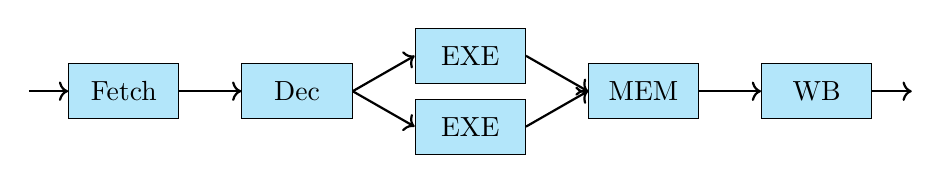
\begin{tikzpicture}[
      stage/.style={draw, fill=cyan!30, minimum width=1.4cm, minimum height=0.7cm},
      arr/.style={->, thick}
    ]
      % Pipeline stages
      \node[stage] (fetch) at (0,0) {Fetch};
      \node[stage] (dec) at (2.2,0) {Dec};
      \node[stage] (exe1) at (4.4,0.45) {EXE};
      \node[stage] (exe2) at (4.4,-0.45) {EXE};
      \node[stage] (mem) at (6.6,0) {MEM};
      \node[stage] (wb) at (8.8,0) {WB};

      % Arrows between stages
      \draw[arr] ([xshift=-0.5cm]fetch.west) -- (fetch.west);
      \draw[arr] (fetch) -- (dec);
      \draw[arr] (dec.east) -- (exe1.west);
      \draw[arr] (dec.east) -- (exe2.west);
      \draw[arr] (exe1.east) -- (mem.west);
      \draw[arr] (exe2.east) -- (mem.west);
      \draw[arr] (mem) -- (wb);
      \draw[arr] (wb.east) -- ([xshift=0.5cm]wb.east);
    \end{tikzpicture}
  \end{center}

  \vspace{0.3cm}
  \begin{itemize}
    \item \textbf{Getting IPC $> 1$ requires to fetch, decode, exe, and retire $>1$ instruction per clock:}
  \end{itemize}

  \begin{center}
    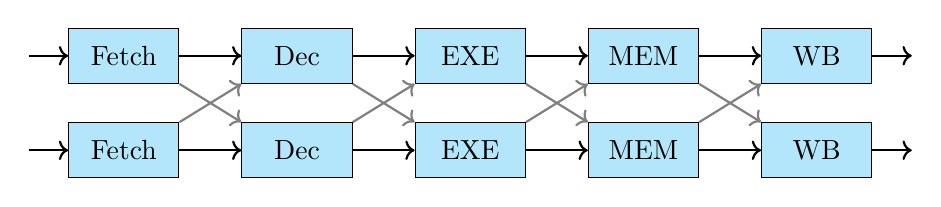
\begin{tikzpicture}[
      stage/.style={draw, fill=cyan!30, minimum width=1.4cm, minimum height=0.7cm},
      arr/.style={->, thick},
      cross/.style={->, gray, thick}
    ]
      % Top pipeline
      \node[stage] (fetch1) at (0,0) {Fetch};
      \node[stage] (dec1) at (2.2,0) {Dec};
      \node[stage] (exe1) at (4.4,0) {EXE};
      \node[stage] (mem1) at (6.6,0) {MEM};
      \node[stage] (wb1) at (8.8,0) {WB};

      % Bottom pipeline
      \node[stage] (fetch2) at (0,-1.2) {Fetch};
      \node[stage] (dec2) at (2.2,-1.2) {Dec};
      \node[stage] (exe2) at (4.4,-1.2) {EXE};
      \node[stage] (mem2) at (6.6,-1.2) {MEM};
      \node[stage] (wb2) at (8.8,-1.2) {WB};

      % Top pipeline arrows
      \draw[arr] ([xshift=-0.5cm]fetch1.west) -- (fetch1.west);
      \draw[arr] (fetch1) -- (dec1);
      \draw[arr] (dec1) -- (exe1);
      \draw[arr] (exe1) -- (mem1);
      \draw[arr] (mem1) -- (wb1);
      \draw[arr] (wb1.east) -- ([xshift=0.5cm]wb1.east);

      % Bottom pipeline arrows
      \draw[arr] ([xshift=-0.5cm]fetch2.west) -- (fetch2.west);
      \draw[arr] (fetch2) -- (dec2);
      \draw[arr] (dec2) -- (exe2);
      \draw[arr] (exe2) -- (mem2);
      \draw[arr] (mem2) -- (wb2);
      \draw[arr] (wb2.east) -- ([xshift=0.5cm]wb2.east);

      % Cross-pipeline arrows (gray)
      \draw[cross] (fetch1.south east) -- (dec2.north west);
      \draw[cross] (fetch2.north east) -- (dec1.south west);
      \draw[cross] (dec1.south east) -- (exe2.north west);
      \draw[cross] (dec2.north east) -- (exe1.south west);
      \draw[cross] (exe1.south east) -- (mem2.north west);
      \draw[cross] (exe2.north east) -- (mem1.south west);
      \draw[cross] (mem1.south east) -- (wb2.north west);
      \draw[cross] (mem2.north east) -- (wb1.south west);
    \end{tikzpicture}
  \end{center}
\end{frame}


\begin{frame}{Misprediction Penalty in a Superscalar CPU}
  \begin{itemize}
    \item \textbf{Assume}
    \begin{itemize}
      \item $\frac{1}{100}$ instruction is a mispredicted jump (MPI = 1\%)
      \item Flush penalty of 5 cycles
    \end{itemize}
    
    \vspace{0.5cm}
    
    \item \textbf{For IPC = 2}
    \begin{itemize}
      \item Flush every $\frac{100}{2} = 50$ cycles
      \item 5 cycles flush penalty every 50 cycles $\Rightarrow$ \alert{10\% performance hit}
    \end{itemize}
    
    \vspace{0.5cm}
    
    \item \textbf{For IPC = 1}
    \begin{itemize}
      \item Flush every $\frac{100}{1} = 100$ cycles
      \item 5 cycles flush penalty per 100 cycles $\Rightarrow$ \alert{5\% performance hit}
    \end{itemize}
    
    \vspace{0.5cm}
    
    \item \alert{Flush penalty increases as the machine is deeper and wider}
  \end{itemize}
\end{frame}

\begin{frame}{Extract More ILP}
  \begin{itemize}
    \item \textbf{ILP -- Instruction Level Parallelism}
    \begin{itemize}
      \item Program parallelism is determined by instruction dependencies
      \item Only independent instructions can execute in parallel
      \item Fully dependent code (each instruction depends on previous) $\Rightarrow$ ILP = 1
      \begin{itemize}
        \item More HW does not help
      \end{itemize}
    \end{itemize}

    \item \textbf{Adjacent instructions are usually dependent}
    \begin{itemize}
      \item In-order superscalar: adding more execution units yields diminishing returns
      \item 2nd unit has lower utilization than 1st, 3rd even lower (blocked by dependencies)
    \end{itemize}

    \item \textbf{Cache misses stall execution} -- dependent instructions wait for missed loads

    \item \textbf{Compilers are limited to basic blocks} and unaware of cache misses

    \item \textbf{Solution: Out-Of-Order Execution}
    \begin{itemize}
      \item Find independent instructions further ahead in the program
      \item Execute based on data readiness, not program order
      \item Maintain original program semantics
    \end{itemize}
  \end{itemize}
\end{frame}

\begin{frame}{Data Flow Analysis}
  \begin{tikzpicture}[
    % Common styles
    code/.style={font=\small\ttfamily, anchor=west},
    titlestyle/.style={font=\small\bfseries},
    inst/.style={circle, draw, minimum size=0.5cm, font=\small, inner sep=1pt},
    dep/.style={->, thick},
    exec/.style={draw, thick, minimum height=0.35cm, minimum width=0.5cm, font=\tiny, inner sep=2pt},
    i1exec/.style={exec, fill=blue!30, minimum width=1.2cm},
    i2exec/.style={exec, fill=green!30},
    i3exec/.style={exec, fill=yellow!30},
    i4exec/.style={exec, fill=orange!30},
    i5exec/.style={exec, fill=purple!30},
    i6exec/.style={exec, fill=red!30},
  ]
    % === LEFT COLUMN: Example code ===
    \node[titlestyle, anchor=west] at (-1,0.3) {Example:};
    \node[code] (line1) at (-1,-0.3) {(1) \textcolor{r1color}{r1} $\leftarrow$ r4 / r7};
    \node[code] at (-1,-0.8) {(2) \textcolor{r8color}{r8} $\leftarrow$ \textcolor{r1color}{r1} + r2};
    \node[code] at (-1,-1.3) {(3) \textcolor{r5color}{r5} $\leftarrow$ r5 + 1};
    \node[code] at (-1,-1.8) {(4) \textcolor{r6color}{r6} $\leftarrow$ r6 - r3};
    \node[code] at (-1,-2.3) {(5) \textcolor{r4color}{r4} $\leftarrow$ \textcolor{r5color}{r5} + \textcolor{r6color}{r6}};
    \node[code] at (-1,-2.8) {(6) r7 $\leftarrow$ \textcolor{r8color}{r8} * \textcolor{r4color}{r4}};

    % Callout for divide - positioned relative to line1, pointing to /
    \node[ellipse callout, draw, fill=blue!10,
          callout absolute pointer={($(line1.east)+(-0.3cm,2mm)$)},
          font=\scriptsize, align=center]
          at ($(line1.north)+(0.5cm,1cm)$)
          {Assume divide\\takes multiple cycles};

    % === RIGHT COLUMN: Data Flow Graph ===
    \begin{scope}[shift={(5.5,0.8)}]
      \node[titlestyle] at (1.2,0.3) {Data Flow Graph};
      % Graph nodes
      \node[inst] (i1) at (0,-0.5) {1};
      \node[inst] (i3) at (1.2,-0.5) {3};
      \node[inst] (i4) at (2.4,-0.5) {4};
      \node[inst] (i2) at (0.6,-1.4) {2};
      \node[inst] (i5) at (1.8,-1.4) {5};
      \node[inst] (i6) at (1.2,-2.3) {6};
      % Dependencies
      \draw[dep] (i1) -- node[left, font=\scriptsize] {\textcolor{r1color}{r1}} (i2);
      \draw[dep] (i3) -- node[left, font=\scriptsize] {\textcolor{r5color}{r5}} (i5);
      \draw[dep] (i4) -- node[right, font=\scriptsize] {\textcolor{r6color}{r6}} (i5);
      \draw[dep] (i2) -- node[left, font=\scriptsize] {\textcolor{r8color}{r8}} (i6);
      \draw[dep] (i5) -- node[right, font=\scriptsize] {\textcolor{r4color}{r4}} (i6);
    \end{scope}

    % === BOTTOM LEFT: In-order execution (appears on click) ===
    \only<2->{
    \begin{scope}[shift={(4,-3.8)}, node distance=1pt]
      \node[i1exec] (io1) at (0,0) {1};
      \node[i2exec, right=of io1] (io2) {2};
      \node[i3exec, below=of io2] (io3) {3};
      \node[i4exec, below=of io3] (io4) {4};
      \node[i5exec, right=of io2] (io5) {5};
      \node[i6exec, right=of io5] (io6) {6};
      \draw[->] ([yshift=-2mm]io1.west |- io4.south) -- ([yshift=-2mm]io6.east |- io4.south) node[right, font=\tiny] {t};
      % Title closer to the diagram
      \node[titlestyle] at (0.8,0.5) {In-Order Execution};
    \end{scope}

    % Callout for in-order - positioned to the left, pointing to instruction 2
    \node[ellipse callout, draw, fill=red!10,
          callout absolute pointer={(io2.west)},
          font=\tiny, text width=3cm, align=center, anchor=east]
          at ($(io1.west)+(-0.3cm,-0.8cm)$)
          {(2) depends on (1), so (3) and (4) must wait even though they're independent of (1)};
    }

    % === BOTTOM RIGHT: Out-of-order execution (appears on second click) ===
    \only<3->{
    \begin{scope}[shift={(9,-3.8)}, node distance=1pt]
      \node[i1exec] (ooo1) at (0,0) {1};
      \node[i3exec, below=1pt of ooo1.south west, anchor=north west] (ooo3) {3};
      \node[i4exec, below=of ooo3] (ooo4) {4};
      \node[i5exec, right=of ooo3] (ooo5) {5};
      \node[i2exec, right=of ooo1] (ooo2) {2};
      \node[i6exec, right=of ooo2] (ooo6) {6};
      \draw[->] ([yshift=-2mm]ooo1.west |- ooo4.south) -- ([yshift=-2mm]ooo6.east |- ooo4.south) node[right, font=\tiny] {t};
      % Title closer to the diagram
      \node[titlestyle] at (0.8,0.5) {Out-of-Order Execution};
    \end{scope}
    }
  \end{tikzpicture}
\end{frame}

\begin{frame}{OOOE: General Scheme}
  \begin{center}
    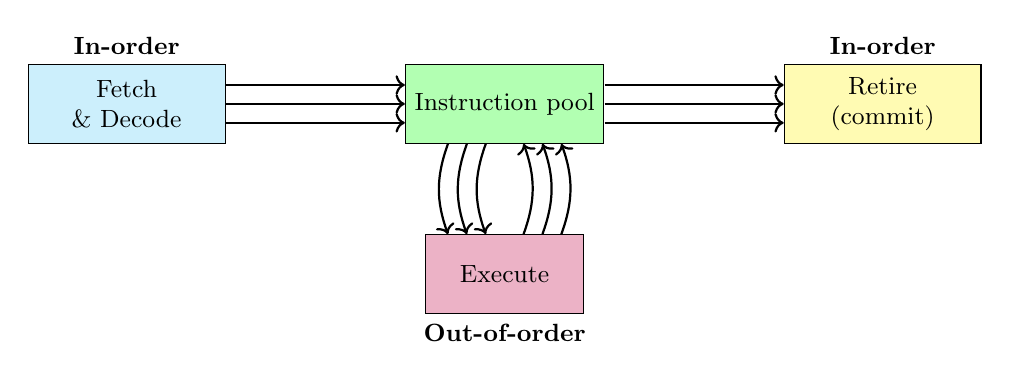
\begin{tikzpicture}[scale=1.2, every node/.style={font=\small},
      fetchblock/.style={rectangle, draw, fill=cyan!20, minimum width=2.5cm, minimum height=1cm},
      block/.style={rectangle, draw, fill=yellow!30, minimum width=2.5cm, minimum height=1cm},
      pool/.style={rectangle, draw, fill=green!30, minimum width=2.5cm, minimum height=1cm},
      exe/.style={rectangle, draw, fill=purple!30, minimum width=2cm, minimum height=1cm}]

      % Blocks
      \node[fetchblock,align=center] (fetch) at (0,0) {Fetch \\\& Decode};
      \node[pool] (pool) at (4,0) {Instruction pool};
      \node[exe] (exec) at (4,-1.8) {Execute};
      \node[block,align=center] (retire) at (8,0) {Retire\\(commit)};
      
      % Arrows with multiple lines
      \draw[->, thick] ([yshift=2mm]fetch.east) -- ([yshift=2mm]pool.west);
      \draw[->, thick] (fetch.east) -- (pool.west);
      \draw[->, thick] ([yshift=-2mm]fetch.east) -- ([yshift=-2mm]pool.west);

      \foreach \y in {-2mm, 0, 2mm} {
        \draw[->, thick] ([yshift=\y]pool.east) -- ([yshift=\y]retire.west);
      }
      
      % Bidirectional connection pool-execute
      \foreach \x in {-6mm, -4mm, -2mm} {
        \draw[->, thick, bend right=20] ([xshift=\x]pool.south) to ([xshift=\x]exec.north);
      }
      \foreach \x in {6mm, 4mm, 2mm} {
        \draw[<-, thick, bend left=20] ([xshift=\x]pool.south) to ([xshift=\x]exec.north);
      }
      % Labels
      \node[above] at (fetch.north) {\textbf{In-order}};
      \node[above] at (retire.north) {\textbf{In-order}};
      \node[below] at (exec.south) {\textbf{Out-of-order}};
    \end{tikzpicture}
  \end{center}

  \vspace{-1.1cm}

  \begin{itemize}
    \item \textbf{Fetch \& decode instructions in parallel but in-order}
    \begin{itemize}
      \item Fill the Instruction Pool
    \end{itemize}
    
    \item \textbf{Execute ready instructions from the instructions pool}
    \begin{itemize}
      \item All source data ready + needed execution resources available
    \end{itemize}
    
    \item \textbf{Once an instruction is executed}
    \begin{itemize}
      \item Signal all dependent instructions that data is ready
    \end{itemize}
    
    \item \textbf{Commit instructions in parallel but in-order}
    \begin{itemize}
      \item State change (memory, register) and fault/exception handling
    \end{itemize}
  \end{itemize}
\end{frame}

\begin{frame}{Write-After-Write Dependency}
  \begin{columns}
    \begin{column}{0.5\textwidth}
      \textbf{Example Code:} \\
      \begin{tabular}{lll}
        (1) & & \texttt{\textcolor{r1color}{r1} $\leftarrow$ r9/17} \\
        (2) & & \texttt{\textcolor{r2color}{r2} $\leftarrow$ \textcolor{r2color}{r2}+\textcolor{r1color}{r1}} \\
        (3) & & \texttt{\textcolor{orange}{r1} $\leftarrow$ 23} \\
        (4) & & \texttt{\textcolor{r3color}{r3} $\leftarrow$ \textcolor{r3color}{r3}+\textcolor{orange}{r1}} \\
        (5) & & \texttt{jcc L2} \\
        (6) & \texttt{L2:} & \texttt{\textcolor{green}{r1} $\leftarrow$ 35} \\
        (7) & & \texttt{\textcolor{r4color}{r4} $\leftarrow$ \textcolor{r3color}{r3}+\textcolor{green}{r1}} \\
        (8) & & \texttt{\textcolor{blue}{r3} $\leftarrow$ 2} \\
      \end{tabular}
    \end{column}
    
    \begin{column}{0.5\textwidth}
      \begin{block}{WAW Issue}
        If inst (3) is executed before inst (1), r1 ends up having a wrong value.
        
        \vspace{0.3cm}
        
        Called \alert{write-after-write false dependency}:
        
        The order of two writes to the same register is flipped.
      \end{block}
    \end{column}
  \end{columns}
\end{frame}
\begin{frame}{What's Next}
  \begin{itemize}
    \item \textbf{Goal: minimize CPU Time}
    \begin{equation*}
      \text{CPU Time} = \text{clock cycle} \times \text{CPI} \times \text{IC}
    \end{equation*}
    
    \item \textbf{So far we have learned}
    \begin{itemize}
      \item Minimize clock cycle $\Rightarrow$ add more pipe stages
      \item Minimize CPI $\Rightarrow$ use pipeline
      \item Minimize IC $\Rightarrow$ architecture
    \end{itemize}

    \item \textbf{In a pipelined CPU}
    \begin{itemize}
      \item CPI w/o hazards is 1
      \item CPI with hazards is $> 1$
    \end{itemize}

    \item \textbf{Adding more pipe stages reduces clock cycle but increases CPI}
    \begin{itemize}
      \item Higher penalty due to control hazards
      \item More data hazards
    \end{itemize}

    \item \alert{What can we do? Further reduce the CPI!}
  \end{itemize}
\end{frame}

\begin{frame}{A Superscalar CPU}
  \begin{itemize}
    \item \textbf{Duplicating HW in one pipe stage won't help}
    \begin{itemize}
      \item e.g., have 2 ALUs
      \item the bottleneck moves to other stages
    \end{itemize}
  \end{itemize}

  \begin{center}
    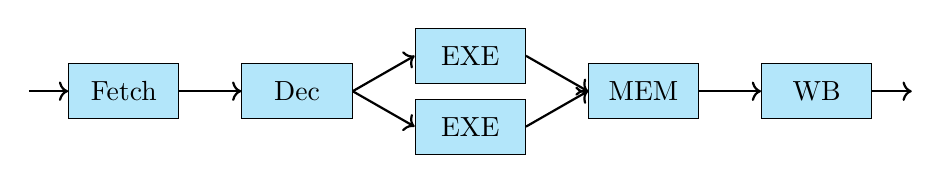
\begin{tikzpicture}[
      stage/.style={draw, fill=cyan!30, minimum width=1.4cm, minimum height=0.7cm},
      arr/.style={->, thick}
    ]
      % Pipeline stages
      \node[stage] (fetch) at (0,0) {Fetch};
      \node[stage] (dec) at (2.2,0) {Dec};
      \node[stage] (exe1) at (4.4,0.45) {EXE};
      \node[stage] (exe2) at (4.4,-0.45) {EXE};
      \node[stage] (mem) at (6.6,0) {MEM};
      \node[stage] (wb) at (8.8,0) {WB};

      % Arrows between stages
      \draw[arr] ([xshift=-0.5cm]fetch.west) -- (fetch.west);
      \draw[arr] (fetch) -- (dec);
      \draw[arr] (dec.east) -- (exe1.west);
      \draw[arr] (dec.east) -- (exe2.west);
      \draw[arr] (exe1.east) -- (mem.west);
      \draw[arr] (exe2.east) -- (mem.west);
      \draw[arr] (mem) -- (wb);
      \draw[arr] (wb.east) -- ([xshift=0.5cm]wb.east);
    \end{tikzpicture}
  \end{center}

  \vspace{0.3cm}
  \begin{itemize}
    \item \textbf{Getting IPC $> 1$ requires to fetch, decode, exe, and retire $>1$ instruction per clock:}
  \end{itemize}

  \begin{center}
    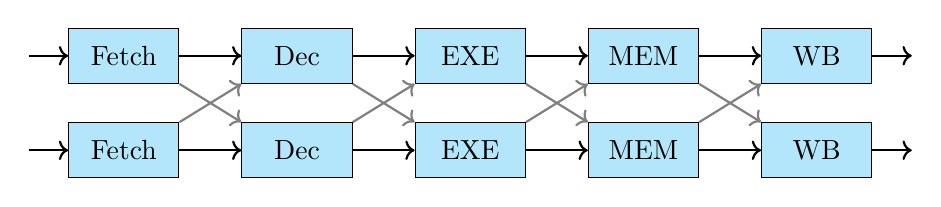
\begin{tikzpicture}[
      stage/.style={draw, fill=cyan!30, minimum width=1.4cm, minimum height=0.7cm},
      arr/.style={->, thick},
      cross/.style={->, gray, thick}
    ]
      % Top pipeline
      \node[stage] (fetch1) at (0,0) {Fetch};
      \node[stage] (dec1) at (2.2,0) {Dec};
      \node[stage] (exe1) at (4.4,0) {EXE};
      \node[stage] (mem1) at (6.6,0) {MEM};
      \node[stage] (wb1) at (8.8,0) {WB};

      % Bottom pipeline
      \node[stage] (fetch2) at (0,-1.2) {Fetch};
      \node[stage] (dec2) at (2.2,-1.2) {Dec};
      \node[stage] (exe2) at (4.4,-1.2) {EXE};
      \node[stage] (mem2) at (6.6,-1.2) {MEM};
      \node[stage] (wb2) at (8.8,-1.2) {WB};

      % Top pipeline arrows
      \draw[arr] ([xshift=-0.5cm]fetch1.west) -- (fetch1.west);
      \draw[arr] (fetch1) -- (dec1);
      \draw[arr] (dec1) -- (exe1);
      \draw[arr] (exe1) -- (mem1);
      \draw[arr] (mem1) -- (wb1);
      \draw[arr] (wb1.east) -- ([xshift=0.5cm]wb1.east);

      % Bottom pipeline arrows
      \draw[arr] ([xshift=-0.5cm]fetch2.west) -- (fetch2.west);
      \draw[arr] (fetch2) -- (dec2);
      \draw[arr] (dec2) -- (exe2);
      \draw[arr] (exe2) -- (mem2);
      \draw[arr] (mem2) -- (wb2);
      \draw[arr] (wb2.east) -- ([xshift=0.5cm]wb2.east);

      % Cross-pipeline arrows (gray)
      \draw[cross] (fetch1.south east) -- (dec2.north west);
      \draw[cross] (fetch2.north east) -- (dec1.south west);
      \draw[cross] (dec1.south east) -- (exe2.north west);
      \draw[cross] (dec2.north east) -- (exe1.south west);
      \draw[cross] (exe1.south east) -- (mem2.north west);
      \draw[cross] (exe2.north east) -- (mem1.south west);
      \draw[cross] (mem1.south east) -- (wb2.north west);
      \draw[cross] (mem2.north east) -- (wb1.south west);
    \end{tikzpicture}
  \end{center}
\end{frame}

\begin{frame}{Misprediction Penalty in a Superscalar CPU}
  \begin{itemize}
    \item \textbf{Assume}
    \begin{itemize}
      \item $\frac{1}{100}$ instruction is a mispredicted jump (MPI = 1\%)
      \item Flush penalty of 5 cycles
    \end{itemize}
    
    \vspace{0.5cm}
    
    \item \textbf{For IPC = 2}
    \begin{itemize}
      \item Flush every $\frac{100}{2} = 50$ cycles
      \item 5 cycles flush penalty every 50 cycles $\Rightarrow$ \alert{10\% performance hit}
    \end{itemize}
    
    \vspace{0.5cm}
    
    \item \textbf{For IPC = 1}
    \begin{itemize}
      \item Flush every $\frac{100}{1} = 100$ cycles
      \item 5 cycles flush penalty per 100 cycles $\Rightarrow$ \alert{5\% performance hit}
    \end{itemize}
    
    \vspace{0.5cm}
    
    \item \alert{Flush penalty increases as the machine is deeper and wider}
  \end{itemize}
\end{frame}

\begin{frame}{Extract More ILP}
  \begin{itemize}
    \item \textbf{ILP -- Instruction Level Parallelism}
    \begin{itemize}
      \item Program parallelism is determined by instruction dependencies
      \item Only independent instructions can execute in parallel
      \item Fully dependent code (each instruction depends on previous) $\Rightarrow$ ILP = 1
      \begin{itemize}
        \item More HW does not help
      \end{itemize}
    \end{itemize}

    \item \textbf{Adjacent instructions are usually dependent}
    \begin{itemize}
      \item In-order superscalar: adding more execution units yields diminishing returns
      \item 2nd unit has lower utilization than 1st, 3rd even lower (blocked by dependencies)
    \end{itemize}

    \item \textbf{Cache misses stall execution} -- dependent instructions wait for missed loads

    \item \textbf{Compilers are limited to basic blocks} and unaware of cache misses

    \item \textbf{Solution: Out-Of-Order Execution}
    \begin{itemize}
      \item Find independent instructions further ahead in the program
      \item Execute based on data readiness, not program order
      \item Maintain original program semantics
    \end{itemize}
  \end{itemize}
\end{frame}

\begin{frame}{Write-After-Write Dependency}
  \begin{columns}
    \begin{column}{0.5\textwidth}
      \textbf{Example Code:} \\
      \begin{tabular}{lll}
        (1) & & \texttt{\textcolor{blue}{r1} $\leftarrow$ r9/17} \\
        (2) & & \texttt{r2 $\leftarrow$ r2+\textcolor{blue}{r1}} \\
        (3) & & \texttt{\textcolor{orange}{r1} $\leftarrow$ 23} \\
        (4) & & \texttt{\textcolor{red}{r3} $\leftarrow$ r3+\textcolor{orange}{r1}} \\
        (5) & & \texttt{jcc L2} \\
        (6) & \texttt{L2:} & \texttt{\textcolor{green}{r1} $\leftarrow$ 35} \\
        (7) & & \texttt{r4 $\leftarrow$ \textcolor{red}{r3}+\textcolor{green}{r1}} \\
        (8) & & \texttt{r3 $\leftarrow$ 2} \\
      \end{tabular}
    \end{column}

    \begin{column}{0.5\textwidth}
      \begin{block}{WAW Issue}
        If inst (3) is executed before inst (1), r1 ends up having a wrong value.
        
        \vspace{0.3cm}
        
        Called \alert{write-after-write false dependency}:
        
        The order of two writes to the same register is flipped.
      \end{block}
    \end{column}
  \end{columns}
\end{frame}

\begin{frame}{WAW False Dependency}
  \begin{columns}
    \begin{column}{0.5\textwidth}
      \textbf{Example Code (reordered):} \\
      \begin{tabular}{lll}
        (3) & & \texttt{\textcolor{orange}{r1\tikzmark{r1dest}} $\leftarrow$ 23} \\
        (1) & & \texttt{\textcolor{blue}{r1\tikzmark{r1blue}} $\leftarrow$ r9/17} \\
        (2) & & \texttt{r2 $\leftarrow$ r2+\textcolor{blue}{r1}} \\
        & & \\
        (4) & & \texttt{\textcolor{red}{r3} $\leftarrow$ r3+\textcolor{orange}{\tikzmark{r1use}r1}} \\
        (5) & & \texttt{jcc L2} \\
        (6) & \texttt{L2:} & \texttt{\textcolor{green}{r1} $\leftarrow$ 35} \\
        (7) & & \texttt{r4 $\leftarrow$ \textcolor{red}{r3}+\textcolor{green}{r1}} \\
        (8) & & \texttt{r3 $\leftarrow$ 2} \\
      \end{tabular}
    \end{column}

    \begin{column}{0.5\textwidth}
      % Arrow showing dependency using tikzmark and callout
      \begin{tikzpicture}[overlay, remember picture]
        \draw[->, thick, orange, dashed] ([xshift=0mm, yshift=1mm]pic cs:r1dest) to[out=0, in=90] ([xshift=2mm, yshift=3mm]pic cs:r1use);
        \draw[->, thick, blue] ([xshift=0mm, yshift=1mm]pic cs:r1blue) -- ([xshift=0mm, yshift=3mm]pic cs:r1use);

        % Callout for specific example positioned relative to r1dest
        \node[rectangle callout, draw=orange, fill=orange!10, thick, align=left, text width=4.5cm,
              font=\small, anchor=west, callout absolute pointer={([xshift=5mm, yshift=2mm]pic cs:r1use)}]
          at ([xshift=3.5cm, yshift=1.3cm]pic cs:r1use)
          {Instruction (4) must use \textcolor{orange}{r1} from instruction (3), not from instruction (1)};
      \end{tikzpicture}

      \vspace{3cm}

      \pause

      \begin{alertblock}{Write-After-Write (WAW)}
        \alert{WAW is a \emph{false dependency}}

        \vspace{0.2cm}

        Not a real data dependency, but an artifact of OOO execution when multiple writes target the same register.
      \end{alertblock}
    \end{column}
  \end{columns}
\end{frame}

\section{Register Renaming}

\begin{frame}{Speculative Execution}
  \begin{columns}
    \begin{column}{0.45\textwidth}
      \textbf{Example Code:} \\
      \begin{tabular}{lll}
        (3) & & \texttt{\textcolor{orange}{r1} $\leftarrow$ 23} \\
        (1) & & \texttt{\textcolor{blue}{r1} $\leftarrow$ r9/17} \\
        (2) & & \texttt{r2 $\leftarrow$ r2+\textcolor{blue}{r1}} \\
        (4) & & \texttt{\textcolor{red}{r3} $\leftarrow$ r3+\textcolor{orange}{r1}} \\
        (5) & & \texttt{jcc L2} \\
        \rowcolor{pink!30} (6) & \texttt{L2:} & \texttt{\textcolor{green}{r1} $\leftarrow$ 35} \\
        \rowcolor{pink!30} (7) & & \texttt{r4 $\leftarrow$ \textcolor{red}{r3}+\textcolor{green}{r1}} \\
        \rowcolor{pink!30} (8) & & \texttt{r3 $\leftarrow$ 2} \\
      \end{tabular}
    \end{column}
    
    \begin{column}{0.55\textwidth}
      \begin{block}{OOO Speculative Execution}
        \small
        \textbf{Every 5th instruction is a branch} $\Rightarrow$ must continue fetching along \textcolor{green}{predicted path} to fill instruction pool.
        
        Without speculation: limited to finding independent instructions only until next branch.
        
        \alert{Speculative Execution:} Execute instructions from predicted path before branch resolution.
        
        Example: inst (6) can execute before inst (1).
        
        If mispredicted: must undo speculatively executed instructions.
      \end{block}
    \end{column}
  \end{columns}
\end{frame}

\begin{frame}{WAR False Dependency}
  \begin{columns}
    \begin{column}{0.5\textwidth}
      \textbf{Example Code (reordered):} \\
      \begin{tabular}{lll}
        (3) & & \texttt{\textcolor{orange}{r1} $\leftarrow$ 23} \\
        (1) & & \texttt{\textcolor{blue}{r1} $\leftarrow$ r9/17} \\
        (2) & & \texttt{r2 $\leftarrow$ r2+\textcolor{blue}{r1}} \\
        & & \\
        (4) & & \texttt{\textcolor{red}{r3\tikzmark{r3dest}} $\leftarrow$ r3+\textcolor{orange}{r1}} \\
        (5) & & \texttt{jcc L2} \\
        (6) & \texttt{L2:} & \texttt{\textcolor{green}{r1} $\leftarrow$ 35} \\
        (8) & & \texttt{\textcolor{blue}{r3\tikzmark{r3write}} $\leftarrow$ 2} \\
        (7) & & \texttt{r4 $\leftarrow$ \textcolor{red}{\tikzmark{r3read}r3}+\textcolor{green}{r1}} \\
      \end{tabular}
    \end{column}

    \begin{column}{0.5\textwidth}
      % Arrow showing dependency using tikzmark and callout
      \begin{tikzpicture}[overlay, remember picture]
        \draw[->, thick, red, dashed] ([xshift=0mm, yshift=1mm]pic cs:r3dest) to[out=0, in=90] ([xshift=2mm, yshift=3mm]pic cs:r3read);
        \draw[->, thick, blue] ([xshift=1mm, yshift=0mm]pic cs:r3write) -- ([xshift=-1mm, yshift=3mm]pic cs:r3read);

        % Callout for specific example positioned relative to r3read
        \node[rectangle callout, draw=red, fill=red!10, thick, align=left, text width=4.5cm,
              font=\small, anchor=west, callout absolute pointer={([xshift=5mm, yshift=2mm]pic cs:r3read)}]
          at ([xshift=4cm, yshift=4.5cm]pic cs:r3read)
          {Instruction (7) must read \textcolor{red}{r3} before instruction (8) overwrites it};
      \end{tikzpicture}

      \vspace{3cm}

      \pause

      \begin{alertblock}{Write-After-Read (WAR)}
        \alert{WAR is a \emph{false dependency}}

        \vspace{0.2cm}

        Not a real data dependency, but an artifact of OOO execution when a write happens before a read of the old value.
      \end{alertblock}
    \end{column}
  \end{columns}
\end{frame}

\begin{frame}{Register Renaming: Overview}
  \begin{itemize}
    \item \textbf{Physical register pool:} Maps architectural registers to physical registers
    
    \item \textbf{Allocation (in-order):}
    \begin{enumerate}
      \item If instruction writes Rx $\rightarrow$ allocate free physical register PRi
      \item Update mapping: Rx $\mapsto$ PRi
      \item Rename sources to their mapped physical registers
    \end{enumerate}
    
    \item \textbf{Execution (out-of-order):}
    \begin{itemize}
      \item Execute when sources ready \& resources available
      \item Write result to PRi (not Rx)
    \end{itemize}
    
    \item \textbf{Commit (in-order):}
    \begin{itemize}
      \item Copy PRi $\rightarrow$ Rx
      \item If Rx still maps to PRi: set mapping to architectural
      \item Return PRi to free pool
    \end{itemize}
  \end{itemize}
\end{frame}

\begin{frame}{Register Renaming: Example}
  \begin{center}
    \begin{tikzpicture}[font=\small]
      \matrix[
        matrix of nodes,
        ampersand replacement=\&,
        row sep=-0.2em,
        column sep=0.3em,
        nodes={anchor=base west, inner sep=2pt, align=left},
        column 1/.style={nodes={minimum width=1.5em}},
        column 2/.style={nodes={minimum width=1.5em}},
        column 3/.style={nodes={text width=6em}},
        column 4/.style={nodes={minimum width=3em}},
        column 5/.style={nodes={text width=7em}},
      ] (m) {
        \& \& |[font=\small\bfseries]| Original \& |[font=\small\bfseries]| Renaming \& |[font=\small\bfseries]| Renamed \\
        (1) \& \& \textcolor{blue}{r1} $\leftarrow$ 17 \& r1:pr1 \& \textcolor{blue}{pr1} $\leftarrow$ 17 \\
        (2) \& \& \textcolor{violet}{r2} $\leftarrow$ r2+\textcolor{blue}{r1} \& r2:pr2 \& \textcolor{violet}{pr2} $\leftarrow$ r2+\textcolor{blue}{pr1} \\
        (3) \& \& \textcolor{orange}{r1} $\leftarrow$ 23 \& \only<2->{r1:pr3} \& \only<2->{\textcolor{orange}{pr3} $\leftarrow$ 23} \\
        (4) \& \& \textcolor{red}{r3} $\leftarrow$ r3+\textcolor{orange}{r1} \& \only<2->{r3:pr4} \& \only<2->{\textcolor{red}{pr4} $\leftarrow$ r3+\textcolor{orange}{pr3}} \\
        (5) \& \& jcc L2 \& \& \\
        (6) \& L2: \& \textcolor{green}{r1} $\leftarrow$ 35 \& \only<3->{r1:pr5} \& \only<3->{\textcolor{green}{pr5} $\leftarrow$ 35} \\
        (7) \& \& r4 $\leftarrow$ \textcolor{red}{r3}+\textcolor{green}{r1} \& \only<3->{r4:pr6} \& \only<3->{pr6 $\leftarrow$ \textcolor{red}{pr4}+\textcolor{green}{pr5}} \\
        (8) \& \& \textcolor{blue}{r3} $\leftarrow$ 2 \& \only<3->{r3:pr7} \& \only<3->{\textcolor{blue}{pr7} $\leftarrow$ 2} \\
      };
      % Callout note pointing to instruction (2): r2 <- r2+r1
      \only<1>{
        \node[rectangle callout, callout absolute pointer={([xshift=-5mm]m-3-3.east)}, fill=yellow!20, draw=yellow!60!black, rounded corners=2pt, font=\scriptsize, text width=4.5cm, align=left, anchor=north west] at ($(m-5-4.west)+(0cm,0.0cm)$) {
          \textbf{Note:} When r2 is both source and destination: \textbf{read first} (using current mapping), then \textbf{write to new} physical register (update mapping).
        };
      }
    \end{tikzpicture}
  \end{center}

  \vspace{0.2cm}
  \begin{center}
    \begin{tabular}{|c|c|c|c|c|}
      \hline
      & r1 & r2 & r3 & r4 \\
      \hline
      Register mapping &
        \only<1>{\textcolor{blue}{pr1}}\only<2>{\textcolor{orange}{pr3}}\only<3->{\textcolor{green}{pr5}} &
        \textcolor{violet}{pr2} &
        \only<1>{r3}\only<2>{\textcolor{red}{pr4}}\only<3->{\textcolor{blue}{pr7}} &
        \only<1-2>{r4}\only<3->{pr6} \\
      \hline
    \end{tabular}
  \end{center}

  \only<2->{\begin{center}
    \colorbox{green!30}{Each instruction uses the correct sources, regardless of the execution order}
  \end{center}}
\end{frame}

\begin{frame}{Misprediction -- Flushing Speculative Work}
  \vspace{-0.5cm}
  \begin{center}
    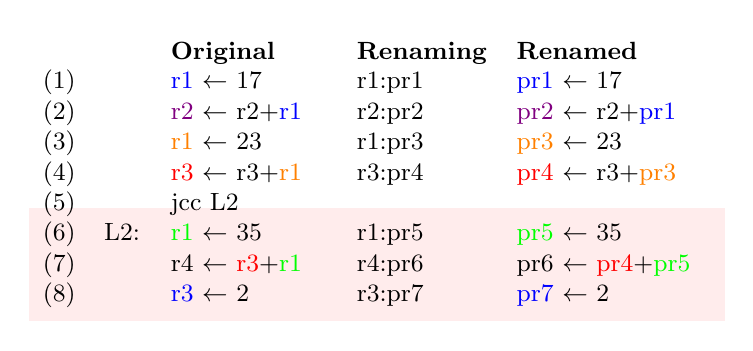
\begin{tikzpicture}[font=\small]
      \matrix[
        matrix of nodes,
        ampersand replacement=\&,
        row sep=-0.2em,
        column sep=0.3em,
        nodes={anchor=base west, inner sep=2pt, align=left},
        column 1/.style={nodes={minimum width=1.5em}},
        column 2/.style={nodes={minimum width=1.5em}},
        column 3/.style={nodes={text width=6em}},
        column 4/.style={nodes={minimum width=3em}},
        column 5/.style={nodes={text width=7em}},
      ] (m) {
        \& \& |[font=\small\bfseries]| Original \& |[font=\small\bfseries]| Renaming \& |[font=\small\bfseries]| Renamed \\
        (1) \& \& \textcolor{blue}{r1} $\leftarrow$ 17 \& r1:pr1 \& \textcolor{blue}{pr1} $\leftarrow$ 17 \\
        (2) \& \& \textcolor{violet}{r2} $\leftarrow$ r2+\textcolor{blue}{r1} \& r2:pr2 \& \textcolor{violet}{pr2} $\leftarrow$ r2+\textcolor{blue}{pr1} \\
        (3) \& \& \textcolor{orange}{r1} $\leftarrow$ 23 \& r1:pr3 \& \textcolor{orange}{pr3} $\leftarrow$ 23 \\
        (4) \& \& \textcolor{red}{r3} $\leftarrow$ r3+\textcolor{orange}{r1} \& r3:pr4 \& \textcolor{red}{pr4} $\leftarrow$ r3+\textcolor{orange}{pr3} \\
        (5) \& \& jcc L2 \& \& \\
        (6) \& L2: \& \textcolor{green}{r1} $\leftarrow$ 35 \& r1:pr5 \& \textcolor{green}{pr5} $\leftarrow$ 35 \\
        (7) \& \& r4 $\leftarrow$ \textcolor{red}{r3}+\textcolor{green}{r1} \& r4:pr6 \& pr6 $\leftarrow$ \textcolor{red}{pr4}+\textcolor{green}{pr5} \\
        (8) \& \& \textcolor{blue}{r3} $\leftarrow$ 2 \& r3:pr7 \& \textcolor{blue}{pr7} $\leftarrow$ 2 \\
      };
      % Pink background for speculative rows (6,7,8)
      \begin{scope}[on background layer]
        \node[fit=(m-7-1)(m-9-5), fill=pink!30, inner sep=3pt] {};
      \end{scope}
    \end{tikzpicture}
  \end{center}

  \vspace{-0.2cm}
  \begin{center}
    \begin{tabular}{|c|c|c|c|c|}
      \hline
      & r1 & r2 & r3 & r4 \\
      \hline
      Register mapping & \textcolor{orange}{pr3} & \textcolor{violet}{pr2} & \textcolor{red}{pr4} & r4 \\
      \hline
    \end{tabular}
  \end{center}

  \vspace{-0.3cm}
  \begin{center}
    \colorbox{blue!15}{\parbox{0.9\textwidth}{If the predicted branch path turns out to be wrong, the instructions following the branch are flushed \textbf{before they are committed} $\Rightarrow$ the architectural state is not changed}}
  \end{center}
\end{frame}

\begin{frame}{Misprediction -- Register Mapping Challenge}
  \vspace{-0.4cm}
  \begin{center}
    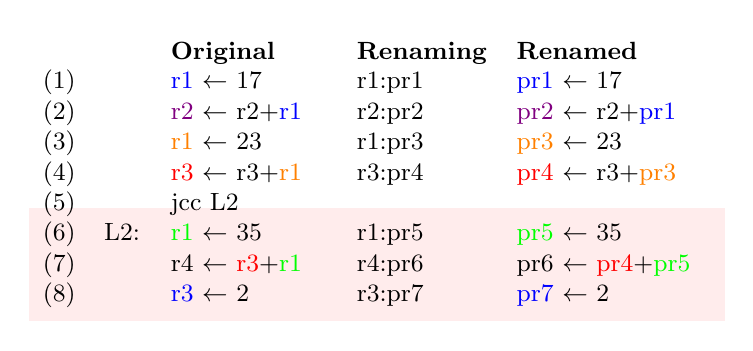
\begin{tikzpicture}[font=\small]
      \matrix[
        matrix of nodes,
        ampersand replacement=\&,
        row sep=-0.2em,
        column sep=0.3em,
        nodes={anchor=base west, inner sep=2pt, align=left},
        column 1/.style={nodes={minimum width=1.5em}},
        column 2/.style={nodes={minimum width=1.5em}},
        column 3/.style={nodes={text width=6em}},
        column 4/.style={nodes={minimum width=3em}},
        column 5/.style={nodes={text width=7em}},
      ] (m) {
        \& \& |[font=\small\bfseries]| Original \& |[font=\small\bfseries]| Renaming \& |[font=\small\bfseries]| Renamed \\
        (1) \& \& \textcolor{blue}{r1} $\leftarrow$ 17 \& r1:pr1 \& \textcolor{blue}{pr1} $\leftarrow$ 17 \\
        (2) \& \& \textcolor{violet}{r2} $\leftarrow$ r2+\textcolor{blue}{r1} \& r2:pr2 \& \textcolor{violet}{pr2} $\leftarrow$ r2+\textcolor{blue}{pr1} \\
        (3) \& \& \textcolor{orange}{r1} $\leftarrow$ 23 \& r1:pr3 \& \textcolor{orange}{pr3} $\leftarrow$ 23 \\
        (4) \& \& \textcolor{red}{r3} $\leftarrow$ r3+\textcolor{orange}{r1} \& r3:pr4 \& \textcolor{red}{pr4} $\leftarrow$ r3+\textcolor{orange}{pr3} \\
        (5) \& \& jcc L2 \& \& \\
        (6) \& L2: \& \textcolor{green}{r1} $\leftarrow$ 35 \& r1:pr5 \& \textcolor{green}{pr5} $\leftarrow$ 35 \\
        (7) \& \& r4 $\leftarrow$ \textcolor{red}{r3}+\textcolor{green}{r1} \& r4:pr6 \& pr6 $\leftarrow$ \textcolor{red}{pr4}+\textcolor{green}{pr5} \\
        (8) \& \& \textcolor{blue}{r3} $\leftarrow$ 2 \& r3:pr7 \& \textcolor{blue}{pr7} $\leftarrow$ 2 \\
      };
      % Pink background for speculative rows (6,7,8)
      \begin{scope}[on background layer]
        \node[fit=(m-7-1)(m-9-5), fill=pink!30, inner sep=3pt] {};
      \end{scope}
    \end{tikzpicture}
  \end{center}

  \vspace{-0.2cm}
  \begin{center}
    \begin{tabular}{|c|c|c|c|c|}
      \hline
      & r1 & r2 & r3 & r4 \\
      \hline
      Register mapping & \colorbox{red!25}{\textcolor{green}{pr5}} & \textcolor{violet}{pr2} & \colorbox{red!25}{\textcolor{blue}{pr7}} & \colorbox{red!25}{pr6} \\
      \hline
    \end{tabular}
  \end{center}

  \vspace{-0.3cm}
  \begin{center}
    \colorbox{blue!15}{\parbox{0.9\textwidth}{The register mapping was already wrongly updated by the wrong path instructions. {\small(e.g., \hyperlink{misprediction-recovery}{checkpointing \& re-renaming})}}}
  \end{center}
\end{frame}

\section{OOO Machine Components}

\begin{frame}{A Superscalar OOO Machine}
  \begin{center}
    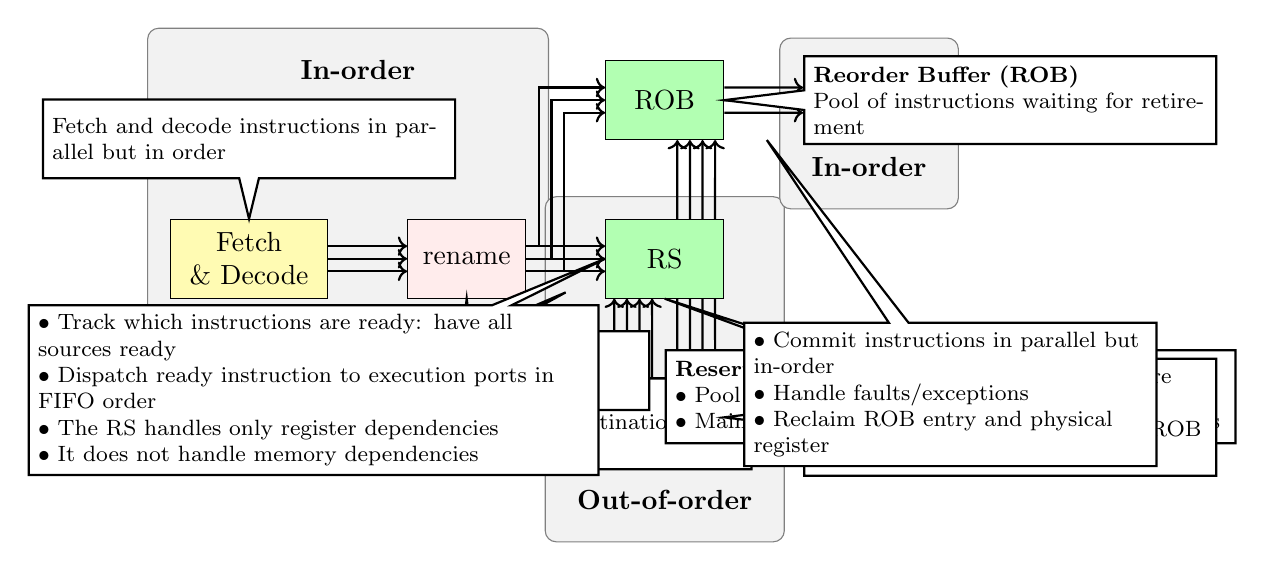
\begin{tikzpicture}[scale=0.8,
      node distance=1cm,
      block/.style={rectangle, draw, fill=yellow!30, minimum width=2cm, minimum height=1cm},
      rename/.style={rectangle, draw, fill=pink!30, minimum width=1.5cm, minimum height=1cm},
      pool/.style={rectangle, draw, fill=green!30, minimum width=1.5cm, minimum height=1cm},
      exe/.style={rectangle, draw, fill=purple!30, minimum width=1.5cm, minimum height=1cm},
      retire/.style={rectangle, draw, fill=yellow!30, minimum width=1.5cm, minimum height=1cm},
      calloutbox/.style={rectangle callout, draw, fill=white, thick, align=left,
                         text width=5cm, minimum height=1cm, font=\footnotesize},
      widecalloutbox/.style={calloutbox, text width=6cm},
      verywidecalloutbox/.style={calloutbox, text width=7cm}]

      % Stage 1: Fetch & Decode + rename
      \node[block,align=center] (fetch) at (0,0) {Fetch \\\& Decode};
      \node[rename, right=of fetch] (rename) {rename};

      % Stage 2: Add ROB and RS
      \onslide<2->{
        \node[pool, right=of rename] (rs) {RS};
        \node[pool, above=of rs] (rob) {ROB};
      }

      % Stage 3: Add Execute
      \onslide<3>{
        \node[exe, below=of rs] (execute) {Execute};
        \node[below=0.3cm of execute.south] (outoforder) {\textbf{Out-of-order}};
      }

      % Stage 4: Add Retire
      \onslide<4->{
        \node[retire,align=center, right=of rob] (retire) {Retire\\(commit)};
        \node[below=0.1cm of retire.south] (inorder2) {\textbf{In-order}};
      }

      % In-order label for initial stages
      \onslide<1-2>{
        \node at ($(fetch)!0.5!(rename)+(0,3)$)  (inorder) {\textbf{In-order}};
      }

      % Fit background for in-order section
      \onslide<1-2>{
        \node[draw=gray, fill=gray!10, fit=(fetch) (rename) (inorder), inner sep=8pt, rounded corners] (bg1) {};
      }
      \onslide<3>{
        \node[draw=gray, fill=gray!10, fit=(rs) (execute) (outoforder), inner sep=8pt, rounded corners] (bg2) {};
      }
      \onslide<4>{
        \node[draw=gray, fill=gray!10, fit=(retire) (inorder2), inner sep=8pt, rounded corners] (bg3) {};
      }

      % Redraw nodes on top to ensure they're visible
      \node[block,align=center] (fetch) at (0,0) {Fetch \\\& Decode};
      \node[rename, right=of fetch] (rename) {rename};
      \onslide<2->{
        \node[pool, right=of rename] (rs) {RS};
        \node[pool, above=of rs] (rob) {ROB};
      }
      \onslide<3->{
        \node[exe, below=of rs] (execute) {Execute};
      }
      \onslide<3>{
        \node[below=0.3cm of execute.south] (outoforder) {\textbf{Out-of-order}};
      }
      \onslide<4->{
        \node[retire,align=center, right=of rob] (retire) {Retire\\(commit)};
        \node[below=0.1cm of retire.south] (inorder2) {\textbf{In-order}};
      }
      \onslide<1-2>{
        \node at ($(fetch)!0.5!(rename)+(0,3)$)  (inorder) {\textbf{In-order}};
      }

      % Arrows - Stage 1
      \foreach \y in {-2mm, 0, 2mm} {
        \draw[->, thick] ([yshift=\y]fetch.east) -- ([yshift=\y]rename.west);
      }

      % Arrows - Stage 2
      \onslide<2->{
        \foreach \y in {-2mm, 0, 2mm} {
          \draw[->, thick] ([yshift=\y]rename.east) -- ([yshift=\y]rs.west);
        }
        \foreach \y in {-2mm, 0, 2mm} {
          \draw[->, thick] ([yshift=\y,xshift=-\y+4mm]rename.east) |- ([yshift=\y]rob.west);
        }
      }

      % Arrows - Stage 3
      \onslide<3->{
        \foreach \x in {2mm, 4mm, 6mm, 8mm} {
          \draw[->, thick] ([xshift=\x]rs.south) -- ([xshift=\x]execute.north);
        }
        \foreach \x in {-2mm, -4mm, -6mm, -8mm} {
          \draw[<-, thick] ([xshift=\x]rs.south) -- ([xshift=\x]execute.north);
        }
        \foreach \x in {2mm, 4mm, 6mm, 8mm} {
          \draw[->, thick] ([xshift=\x]rs.north) -- ([xshift=\x]rob.south);
        }
      }

      % Arrows - Stage 4
      \onslide<4->{
        \foreach \y in {-2mm, 0, 2mm} {
          \draw[->, thick] ([yshift=\y]rob.east) -- ([yshift=\y]retire.west);
        }
      }

      % Callout annotations - Stage  right1
      \onslide<1>{
        \node[calloutbox, above=0.5cm of fetch, callout absolute pointer={(fetch.north)}]
          (fetch_call)
          {Fetch and decode instructions in parallel but in order};

        \node[verywidecalloutbox, below=of rename, callout absolute pointer={(rename.south)}]
          (rename_call)
          {$\bullet$ Rename sources to physical registers\\
          $\bullet$ Allocate a physical register to the destination\\
          $\bullet$ Update the mapping};
      }

      % Callout annotations - Stage 2
      \onslide<2>{
        \node[calloutbox, right=1cm of rob, callout absolute pointer={(rob.east)}]
          (rob_call)
          {\textbf{Reorder Buffer (ROB)}\\Pool of instructions waiting for retirement};

        \node[verywidecalloutbox, anchor=north west, callout absolute pointer={(rs.south)}]
          at ([yshift=-8mm]rs.south) (rs_call)
          {\textbf{Reservation Stations (RS)}\\$\bullet$ Pool of instructions waiting for execution\\$\bullet$ Maintains per inst. sources ready/not-ready status};

        \node[widecalloutbox, anchor=north, callout absolute pointer={($(rename.south)!0.5!(rs.south)+(0,1mm)$)}]
          at ([yshift=-5mm, xshift=-1cm]rename.south) (rename_call2)
          {Allocate instructions in RS and in ROB};
      }

      % Callout annotations - Stage 3
      \onslide<3>{
        \node[verywidecalloutbox, below left=0.1cm of rs, callout absolute pointer={(rs.west)}]
          (rs_call3)
          {$\bullet$ Track which instructions are ready: have all sources ready\\
          $\bullet$ Dispatch ready instruction to execution ports in FIFO order\\
          $\bullet$ The RS handles only register dependencies \\
          $\bullet$ It does not handle memory dependencies};

        \node[calloutbox, right=of execute, callout absolute pointer={(execute.east)}]
          (execute_call)
          {$\bullet$ Write back value and mark more sources as ready\\
          $\bullet$ Send "exe done" indication to ROB and reclaim RS entry};
      }

      % Callout annotations - Stage 4
      \onslide<4>{
        \node[calloutbox, anchor=north west, callout absolute pointer={($(rob.south)!0.5!(retire.south)$)}]
          at ([yshift=-1cm,xshift=3mm]rs.east) (retire_call)
          {$\bullet$ Commit instructions in parallel but in-order\\
          $\bullet$ Handle faults/exceptions\\
          $\bullet$ Reclaim ROB entry and physical register};
      }
    \end{tikzpicture}
  \end{center}
\end{frame}

\begin{frame}{The Re-order Buffer (ROB)}
  \begin{itemize}
    \item \textbf{Holds instructions from allocation until retirement}
    \begin{itemize}
      \item Maintains program order
    \end{itemize}

    \item \textbf{Provides physical register space for register renaming}
    \begin{itemize}
      \item One physical register per ROB entry
      \item Physical register number = ROB entry number
      \item Each instruction has at most one destination register
      \item Buffers execution results until retirement
    \end{itemize}
  \end{itemize}

  \vspace{0.3cm}
  \centering
  \begin{minipage}{6.5cm}
  \centering
  \textbf{ROB}

  \vspace{0.2cm}
  \footnotesize
  \begin{tabular}{|c|c|c|c|c|}
  \hline
  \rowcolor{cyan!20}
  \textbf{Phys Reg} & \textbf{Alloc} & \multicolumn{2}{c|}{\textbf{Data}} & \textbf{Arch} \\
  \rowcolor{cyan!20}
  \textbf{(ROB\#)} & & \textbf{V} & \textbf{Value} & \textbf{Reg} \\
  \hline
  0 & 1 & 1 & 12H & R2 \\
  \hdashline[2pt/2pt]
  1 & 1 & 1 & 33H & R3 \\
  \hdashline[2pt/2pt]
  2 & 1 & 0 & xxx & R8 \\
  \hdashline[2pt/2pt]
  \dots & \dots & \dots & \dots & \dots \\
  \hdashline[2pt/2pt]
  39 & 0 & x & xxx & XXX \\
  \hline
  \end{tabular}

  \vspace{0.2cm}
  {\footnotesize
  \textbf{Fields:} Phys Reg=Physical register number, Alloc=Entry allocated (1/0), Data V=Data valid (1/0), Arch Reg=Destination architectural register
  }
  \end{minipage}
\end{frame}

\begin{frame}{ARF -- Architectural Register File}
  \begin{itemize}
    \item \textbf{Stores committed architectural register values}
    \begin{itemize}
      \item Contains the architectural state visible to the program
      \item Architectural registers: R0, R1, R2, \dots
    \end{itemize}

    \vspace{0.3cm}

    \item \textbf{Register values updated at retirement}
    \begin{itemize}
      \item Value = result from last committed instruction that wrote to this register
      \item Provides values for instructions when no in-flight rename exists
    \end{itemize}
  \end{itemize}

  \vspace{0.5cm}
  \centering
  \begin{minipage}{4cm}
  \centering
  \textbf{ARF}

  \vspace{0.2cm}
  \small
  \begin{tabular}{|c|c|}
  \hline
  \rowcolor{blue!20}
  \textbf{Arch Reg} & \textbf{Value} \\
  \hline
  R0 & 9AH \\
  \hdashline[2pt/2pt]
  R1 & F34H \\
  \hdashline[2pt/2pt]
  \dots & \dots \\
  \hline
  \end{tabular}
  \end{minipage}
\end{frame}

\begin{frame}{Reservation Station (RS)}
  \begin{itemize}
    \item \textbf{Pool of instructions waiting for execution}
    \begin{itemize}
      \item Holds instruction operation and source operands
      \item Tracks operand readiness (valid flag)
      \item Instructions dispatch to execution units when operands ready
    \end{itemize}
  \end{itemize}

  \vspace{0.3cm}
  \centering
  \begin{minipage}{8cm}
  \centering
  \textbf{RS}

  \vspace{0.2cm}
  \footnotesize
  \begin{tabular}{|c|c|c|c|c|c|c|}
  \hline
  \rowcolor{orange!20}
  \textbf{Entry} & \textbf{op} & \multicolumn{2}{c|}{\textbf{src1}} & \multicolumn{2}{c|}{\textbf{src2}} & \textbf{Pdst} \\
  \rowcolor{orange!20}
  \textbf{Valid} & & \textbf{V} & \textbf{Val} & \textbf{V} & \textbf{Val} & \textbf{(ROB\#)} \\
  \hline
  1 & add & 1 & 97H & 1 & 12H & 37 \\
  \hdashline[2pt/2pt]
  1 & sub & 0 & rob37 & 1 & 33H & 38 \\
  \hline
  \end{tabular}
  \end{minipage}

  \vspace{0.4cm}
  \begin{itemize}
    \item \textbf{Operand value sourcing at allocation:}
  \end{itemize}

  \vspace{0.1cm}
  \centering
  \footnotesize
  \begin{tabular}{|l|c|l|}
    \hline
    \rowcolor{orange!20}
    \textbf{Operand from} & \textbf{Data valid} & \textbf{Get value from} \\
    \hline
    Architectural register & 1 & ARF \\
    \hline
    Physical register (ready) & 1 & ROB \\
    \hline
    Physical register (not ready) & 0 & Wait for broadcast \\
    \hline
  \end{tabular}
\end{frame}

\begin{frame}{Reservation Station (RS) - Operation}
  \begin{itemize}
    \item \textbf{RS maintains operands status ``ready/not-ready''}

    \vspace{0.3cm}

    \item Each cycle, executed instructions make more operands ``ready''
    \begin{itemize}
      \item RS arbitrates the write-back busses between the execution units
      \item RS monitors the write-back buses to capture data needed by awaiting instructions
      \item Data can be bypassed directly from a write-back bus to execution unit
    \end{itemize}

    \vspace{0.3cm}

    \item Instructions for which all operands are ready can be \emph{dispatched} for execution
    \begin{itemize}
      \item Dispatcher chooses which of the \emph{ready} instructions to execute next
      \item Dispatches chosen instructions to Execution Units
    \end{itemize}
  \end{itemize}

  \vspace{0.3cm}
  \centering
  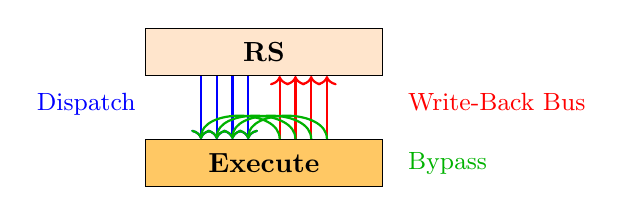
\begin{tikzpicture}
    % RS and Execute blocks
    \node[draw, fill=orange!20, minimum width=3cm, minimum height=0.6cm] (rs) {\textbf{RS}};
    \node[draw, fill=highlightorange, minimum width=3cm, minimum height=0.6cm, below=0.8cm of rs] (execute) {\textbf{Execute}};

    % Arrows from Execute to RS (Write-Back) with increasing xshift
    \foreach \i in {1,2,3,4} {
      \pgfmathsetmacro\shift{\i*2}
      \draw[->, thick, red] ([xshift=\shift mm]execute.north) -- ([xshift=\shift mm]rs.south);
    }

    % Arrows from RS to Execute (Dispatch) with negative xshift
    \foreach \i in {1,2,3,4} {
      \pgfmathsetmacro\shift{-\i*2}
      \draw[->, thick, blue] ([xshift=\shift mm]rs.south) -- ([xshift=\shift mm]execute.north);
    }

    % Curved arrows from Execute (Bypass) with positive xshift to xshift-10mm
    \foreach \i in {1,2,3,4} {
      \pgfmathsetmacro\startshift{\i*2}
      \pgfmathsetmacro\endshift{\i*2-10}
      \draw[->, thick, green!70!black, bend right=90] ([xshift=\startshift mm]execute.north) to ([xshift=\endshift mm]execute.north);
    }

    % Labels with colors matching arrows
    \node[right=0.2cm of execute.east, align=left, font=\small, color=green!70!black] {Bypass};
    \node[align=right, font=\small, color=blue, anchor=north east] at ([yshift=-4mm,xshift=0mm]rs.west) {Dispatch};
    \node[xshift=2mm, align=left, font=\small, color=red, anchor=north west] at ([yshift=-4mm,xshift=0mm]rs.east) {Write-Back Bus};
  \end{tikzpicture}
\end{frame}

\begin{frame}{Getting the Value of a Source Register}
  \textbf{Assume:} Instruction X writes arch register Rj, allocated physical register PRi (ROB entry i)

  \vspace{0.2cm}

  \begin{itemize}
    \item \textbf{On Execution (X completes):}
    \begin{itemize}
      \item Write result to PRi
      \item Broadcast PRi value to all matching sources in RS
    \end{itemize}

    \item \textbf{While Pending (Rj$\rightarrow$PRi mapping active):}
    \begin{itemize}
      \item Subsequent instructions reading Rj use PRi as source
      \item Get value from ROB entry i (marked valid if ready)
    \end{itemize}

    \item \textbf{On Retirement (X commits):}
    \begin{itemize}
      \item Copy PRi value to ARF(Rj)
      \item If Rj still maps to PRi:
      \begin{itemize}
        \item Update RAT: Rj $\rightarrow$ ARF
        \item Future reads of Rj source from ARF until next write
      \end{itemize}
    \end{itemize}
  \end{itemize}
\end{frame}

\begin{frame}{Allocation and Renaming}
  \begin{itemize}
    \item \textbf{Perform register allocation and renaming for $\leq$4 instructions/cyc}

    \item \textbf{Register Alias Table (RAT) maps architectural to physical registers}
    \begin{itemize}
      \item Holds the latest physical register number that updates each architectural register
      \item When allocating an instruction writing to arch register R:
      \begin{itemize}
        \item Map R to the physical register assigned as destination
      \end{itemize}
    \end{itemize}

    \item \textbf{Allocator assigns ROB/RS entries and resolves sources}
    \begin{itemize}
      \item Assigns entry number in ROB and RS
      \item For each source (architectural register):
      \begin{itemize}
        \item Lookup RAT to find latest physical register
        \item Record in RS entry
      \end{itemize}
    \end{itemize}
  \end{itemize}

  \vspace{0.2cm}
  \centering
  \begin{minipage}{5cm}
  \centering
  \textbf{RAT}

  \vspace{0.2cm}
  \small
  \begin{tabular}{|l|c|l|}
  \hline
  \rowcolor{purple!20}
  \textbf{Arch Reg} & \textbf{Phys Reg} & \textbf{Location} \\
  \hline
  R1 & 1 & ARF \\
  \hdashline[2pt/2pt]
  R2 & 19 & ROB \\
  \hdashline[2pt/2pt]
  R3 & 23 & ROB \\
  \hline
  \end{tabular}
  \end{minipage}
\end{frame}

\begin{frame}
  \frametitle<1>{Structure Interaction}
  \frametitle<2>{Register Renaming Example (1)}
  \frametitle<3>{Register Renaming Example (2)}

  \begin{tikzpicture}[font=\tiny, remember picture, overlay]
    % Explanation box in top left corner
    \node[draw, fill=yellow!10, inner sep=5pt, text width=5cm, align=left, anchor=north west] at ([xshift=0.2cm, yshift=-1.5cm]current page.north west) {
      \tiny
      \only<1>{
      \textbf{Instructions Flow:}\\[0.1cm]
      IDQ $\rightarrow$ RAT (decode/rename) $\rightarrow$ ROB \& RS (track \& wait) $\rightarrow$ Execute\\[0.2cm]

      \textbf{Physical Registers:}\\[0.05cm]
      ROB\# entries referenced by:\\
      - RAT: maps arch to phys reg\\
      - RS.Pdst: destination\\
      - RS.srcX: source operands
      }
      \only<2>{
      \textbf{Actions:}\\[0.05cm]
      - \textbf{Read sources BEFORE renaming:} ARF(R1), ROB19(R2)\\
      - Allocate ROB37 for R1\\
      - Update RAT: R1 $\rightarrow$ ROB37\\
      - Add to RS with both operands ready\\
      - ROB37: Alloc=1, Data Valid=0
      }
      \only<3>{
      \textbf{Actions:}\\[0.05cm]
      - \textbf{Read sources BEFORE renaming:} ROB23(R3), ROB37(R1)\\
      - Allocate ROB38 for R1\\
      - Update RAT: R1 $\rightarrow$ ROB38\\
      - Add to RS, \texttt{sub} waits for ROB37\\
      - ROB38: Alloc=1, Data Valid=0
      }
    };
  \end{tikzpicture}

  \centering
  \begin{tikzpicture}[font=\tiny]
    % IDQ at top (always present)
    \node[draw, fill=lightblue, inner sep=5pt] (idq) {\textbf{IDQ}};

    % Instruction node on arrow from IDQ to RAT
    \only<2>{
      \node[draw, fill=green!20, inner sep=3pt, font=\tiny, below right=0.02cm and 0.1cm of idq] (instr1) {\texttt{add R1$\leftarrow$R2,R1}};
    }
    \only<3>{
      \node[draw, fill=green!20, inner sep=3pt, font=\tiny, below right=0.02cm and 0.1cm of idq] (instr2) {\texttt{sub R1$\leftarrow$R3,R1}};
    }

    % RAT below IDQ
    \node[fill=green!10, inner sep=5pt, below=0.4cm of idq] (rat) {
      \begin{minipage}{4cm}
      \centering
      \textbf{RAT}

      \vspace{0.1cm}
      \tiny
      \only<1>{
      \begin{tabular}{|l|c|l|}
      \hline
      \textbf{Arch} & \textbf{Phys} & \textbf{Loc} \\
      \hline
      R1 & xxx & ARF \\
      \hdashline[2pt/2pt]
      R2 & 19 & ROB \\
      \hdashline[2pt/2pt]
      R3 & 23 & ROB \\
      \hline
      \end{tabular}
      }
      \only<2>{
      \begin{tabular}{|l|c|l|}
      \hline
      \textbf{Arch} & \textbf{Phys} & \textbf{Loc} \\
      \hline
      R1 & \textcolor{red}{37} & \textcolor{red}{ROB} \\
      \hdashline[2pt/2pt]
      R2 & 19 & ROB \\
      \hdashline[2pt/2pt]
      R3 & 23 & ROB \\
      \hline
      \end{tabular}
      }
      \only<3>{
      \begin{tabular}{|l|c|l|}
      \hline
      \textbf{Arch} & \textbf{Phys} & \textbf{Loc} \\
      \hline
      R1 & \textcolor{red}{38} & \textcolor{red}{ROB} \\
      \hdashline[2pt/2pt]
      R2 & 19 & ROB \\
      \hdashline[2pt/2pt]
      R3 & 23 & ROB \\
      \hline
      \end{tabular}
      }
      \end{minipage}
    };

    % ROB below and left of RAT
    \node[fill=cyan!10, inner sep=5pt, below=0.8cm of rat.south, anchor=north, xshift=-3.5cm] (rob) {
      \begin{minipage}{4.8cm}
      \centering
      \textbf{ROB}

      \vspace{0.1cm}
      \tiny
      \only<1>{
      \begin{tabular}{|c|c|c|c|c|}
      \hline
      \textbf{Phys Reg} & \textbf{Alloc} & \multicolumn{2}{c|}{\textbf{Data}} & \textbf{Arch} \\
      \textbf{(ROB)} & & \textbf{V} & \textbf{Value} & \textbf{Reg} \\
      \hline
      19 & 1 & 1 & 12H & R2 \\
      \hdashline[2pt/2pt]
      23 & 1 & 1 & 33H & R3 \\
      \hdashline[2pt/2pt]
      37 & 0 & x & xxx & xxx \\
      \hdashline[2pt/2pt]
      38 & 0 & x & xxx & xxx \\
      \hline
      \end{tabular}
      }
      \only<2>{
      \begin{tabular}{|c|c|c|c|c|}
      \hline
      \textbf{Phys Reg} & \textbf{Alloc} & \multicolumn{2}{c|}{\textbf{Data}} & \textbf{Arch} \\
      \textbf{(ROB)} & & \textbf{V} & \textbf{Value} & \textbf{Reg} \\
      \hline
      19 & 1 & 1 & 12H & R2 \\
      \hdashline[2pt/2pt]
      23 & 1 & 1 & 33H & R3 \\
      \hdashline[2pt/2pt]
      \textcolor{red}{37} & \textcolor{red}{1} & \textcolor{red}{0} & \textcolor{red}{xxx} & \textcolor{red}{R1} \\
      \hdashline[2pt/2pt]
      38 & 0 & x & xxx & xxx \\
      \hline
      \end{tabular}
      }
      \only<3>{
      \begin{tabular}{|c|c|c|c|c|}
      \hline
      \textbf{Phys Reg} & \textbf{Alloc} & \multicolumn{2}{c|}{\textbf{Data}} & \textbf{Arch} \\
      \textbf{(ROB)} & & \textbf{V} & \textbf{Value} & \textbf{Reg} \\
      \hline
      19 & 1 & 1 & 12H & R2 \\
      \hdashline[2pt/2pt]
      23 & 1 & 1 & 33H & R3 \\
      \hdashline[2pt/2pt]
      37 & 1 & 0 & xxx & R1 \\
      \hdashline[2pt/2pt]
      \textcolor{red}{38} & \textcolor{red}{1} & \textcolor{red}{0} & \textcolor{red}{xxx} & \textcolor{red}{R1} \\
      \hline
      \end{tabular}
      }
      \end{minipage}
    };

    % RS below and right of RAT
    \node[fill=orange!10, inner sep=5pt, below=0.8cm of rat.south, anchor=north, xshift=3.5cm] (rs) {
      \begin{minipage}{5cm}
      \centering
      \textbf{RS}

      \vspace{0.1cm}
      \tiny
      \only<1>{
      \begin{tabular}{|c|c|c|c|c|c|}
      \hline
      & \multicolumn{2}{c|}{\textbf{src1}} & \multicolumn{2}{c|}{\textbf{src2}} & \textbf{Pdst} \\
      \textbf{op} & \textbf{V} & \textbf{Val} & \textbf{V} & \textbf{Val} & \textbf{(ROB)} \\
      \hline
      -- & -- & -- & -- & -- & -- \\
      \hdashline[2pt/2pt]
      -- & -- & -- & -- & -- & -- \\
      \hline
      \end{tabular}
      }
      \only<2>{
      \begin{tabular}{|c|c|c|c|c|c|}
      \hline
      & \multicolumn{2}{c|}{\textbf{src1}} & \multicolumn{2}{c|}{\textbf{src2}} & \textbf{Pdst} \\
      \textbf{op} & \textbf{V} & \textbf{Val} & \textbf{V} & \textbf{Val} & \textbf{(ROB)} \\
      \hline
      \textcolor{red}{add} & \textcolor{red}{1} & \textcolor{red}{97H} & \textcolor{red}{1} & \textcolor{red}{12H} & \textcolor{red}{37} \\
      \hdashline[2pt/2pt]
      -- & -- & -- & -- & -- & -- \\
      \hline
      \end{tabular}
      }
      \only<3>{
      \begin{tabular}{|c|c|c|c|c|c|}
      \hline
      & \multicolumn{2}{c|}{\textbf{src1}} & \multicolumn{2}{c|}{\textbf{src2}} & \textbf{Pdst} \\
      \textbf{op} & \textbf{V} & \textbf{Val} & \textbf{V} & \textbf{Val} & \textbf{(ROB)} \\
      \hline
      add & 1 & 97H & 1 & 12H & 37 \\
      \hdashline[2pt/2pt]
      \textcolor{red}{sub} & \textcolor{red}{0} & \textcolor{red}{rob37} & \textcolor{red}{1} & \textcolor{red}{33H} & \textcolor{red}{38} \\
      \hline
      \end{tabular}
      }
      \end{minipage}
    };

    % ARF below ROB
    \node[fill=blue!15, inner sep=5pt, below=0.3cm of rob.south, anchor=north] (arf) {
      \begin{minipage}{2cm}
      \centering
      \tiny
      \textbf{ARF}

      \begin{tabular}{|c|c|}
      \hline
      R1 & 97H \\
      \hline
      \end{tabular}
      \end{minipage}
    };

    % Execute below RS
    \node[draw, fill=highlightorange, inner sep=5pt, below=0.5cm of rs.south east, anchor=east] (execute) {\textbf{Execute}};

    % Arrows
    \draw[->, thick] (idq.south) -- (rat.north);
    \draw[->, thick] (rat.south) -- ++(0,-0.3) -| (rob.north);
    \draw[->, thick] (rat.south) -- ++(0,-0.3) -| (rs.north);
    \draw[->, thick] (execute.north) -- (rs.south -| execute.north);
    \draw[->, thick] (execute.west) -| ([xshift=3mm]rob.east) -- (rob.east);

    % Renamed instruction node on arrow from RAT to RS (top right of arrow)
    \only<2>{
      \node[draw, fill=orange!20, inner sep=2pt, font=\tiny, above right=0.4cm and 0.3cm of rs.north west, anchor=south west] (renamed1) {\texttt{add ROB37$\leftarrow$ROB19,ARF1}};
    }
    \only<3>{
      \node[draw, fill=orange!20, inner sep=2pt, font=\tiny, above right=0.4cm and 0.3cm of rs.north west, anchor=south west] (renamed2) {\texttt{sub ROB38$\leftarrow$ROB23,ROB37}};
    }

  \end{tikzpicture}
\end{frame}

\begin{frame}{The Reorder Buffer (ROB)}
  \vspace{-0.5cm}
  \begin{columns}
    \begin{column}{0.65\textwidth}
      \begin{itemize}
        \item<1-> Instructions allocated in-order

        \item<2-> After instruction executes (OOO):
        \begin{itemize}
          \item Mark as \emph{executed} $\Rightarrow$ ready to retire
        \end{itemize}

        \item<3-> Retirement (in-order, oldest first):
        \begin{itemize}
          \item Only after all prior instructions retire
        \end{itemize}
        \item<3-> Upon retirement:
        \begin{itemize}
          \item Copy value from physical to architectural register
          \item Update ARF (Architectural Register File)
          \item Reclaim ROB entry
        \end{itemize}
      \end{itemize}
    \end{column}
    \begin{column}{0.35\textwidth}
      \begin{center}
        \begin{tikzpicture}[font=\tiny,
          E/.style={draw, fill=white, minimum width=1.8cm, minimum height=0.32cm, inner sep=0},
          G/.style={E, fill=green!30},
          N/.style={E, fill=green!50},
          R/.style={E, fill=red!30},
          RR/.style={E, fill=red!60}
        ]
          \matrix[matrix of nodes, ampersand replacement=\&, row sep=-\pgflinewidth,
            nodes={minimum width=1.8cm, minimum height=0.32cm, inner sep=0}
          ] (m) {
            |[E]| \\ |[E]| \\
            |[E]| \\ |[E]| \\ |[E]| \\ |[E]| \\ |[E]| \\ |[E]| \\ |[E]| \\
            |[E]| \\ |[E]| \\ |[E]| \\ |[E]| \\ |[E]| \\ |[E]| \\ |[E]| \\
            |[E]| \\ |[E]| \\ |[E]| \\
          };

          % ROB label
          \node[above=0.1cm of m-1-1, font=\small] {ROB};

          % Stage 1: Allocated (green) + new entries
          \only<1>{
            \foreach \i in {3,...,14} { \node[G] at (m-\i-1) {}; }
            \foreach \i in {15,16,17} { \node[N] at (m-\i-1) {}; }
            \node[fill=green!50, inner sep=2pt, font=\tiny, align=center] at (m-16-1.center) {new\\entries};

            % Labels
            \node[left=0.4cm of m-3-1.west, anchor=east] (retire) {\scriptsize retire};
            \draw[->,thick] (retire) -- (m-3-1.west);
            \node[right=0.1cm of m-3-1.east, anchor=west] {\scriptsize oldest};

            % Faded previous state
            \node[left=0.4cm of m-15-1.west, anchor=east, opacity=0.4] (alloc_old) {\scriptsize alloc};
            \draw[->,thick, opacity=0.4] (alloc_old) -- (m-15-1.west);
            \node[right=0.1cm of m-14-1.east, anchor=west, opacity=0.4] (youngest_old) {\scriptsize youngest};

            % Current state
            \node[left=0.4cm of m-18-1.west, anchor=east] (alloc) {\scriptsize alloc};
            \draw[->,thick] (alloc) -- (m-18-1.west);
            \node[right=0.1cm of m-17-1.east, anchor=west] (youngest) {\scriptsize youngest};

            % Dashed arrows
            \draw[->,dashed,thick] (alloc_old.south) -- (alloc.north);
            \draw[->,dashed,thick] (youngest_old.south) -- (youngest.north);
          }

          % Stage 2: Some executed (red)
          \only<2>{
            \node[G] at (m-3-1) {};
            \foreach \i in {4,5,7,8,10,11,12} { \node[R] at (m-\i-1) {}; }
            \foreach \i in {6,9,13,14,15,16,17} { \node[G] at (m-\i-1) {}; }

            % "Executed" labels
            \node[fill=red!30, inner sep=1pt, font=\tiny] at ($(m-4-1)!0.5!(m-5-1)$) {executed};
            \node[fill=red!30, inner sep=1pt, font=\tiny] at ($(m-7-1)!0.5!(m-8-1)$) {executed};
            \node[fill=red!30, inner sep=1pt, font=\tiny] at (m-11-1.center) {executed};

            % Labels
            \node[left=0.4cm of m-3-1.west, anchor=east] (retire) {\scriptsize retire};
            \draw[->,thick] (retire) -- (m-3-1.west);
            \node[right=0.1cm of m-3-1.east, anchor=west] {\scriptsize oldest};
            \node[left=0.4cm of m-18-1.west, anchor=east] (alloc) {\scriptsize alloc};
            \draw[->,thick] (alloc) -- (m-18-1.west);
            \node[right=0.1cm of m-17-1.east, anchor=west] {\scriptsize youngest};
          }

          % Stage 3: Retirement
          \only<3>{
            \node[RR] at (m-3-1) {};
            \foreach \i in {4,5} { \node[R] at (m-\i-1) {}; }
            \foreach \i in {7,8,10,11,12} { \node[R] at (m-\i-1) {}; }
            \foreach \i in {6,9,13,14,15,16,17} { \node[G] at (m-\i-1) {}; }

            % Fade the top three entries (retired)
            \fill[white, opacity=0.6] (m-3-1.north west) rectangle (m-5-1.south east);
            \node[font=\tiny, opacity=0.8] at (m-4-1.center) {reclaimed};

            % Faded previous state
            \node[left=0.4cm of m-3-1.west, anchor=east, opacity=0.4] (retire_old) {\scriptsize retire};
            \draw[->,thick, opacity=0.4] (retire_old) -- (m-3-1.west);
            \node[right=0.1cm of m-3-1.east, anchor=west, opacity=0.4] (oldest_old) {\scriptsize oldest};

            % Current state (new retire position)
            \node[left=0.4cm of m-6-1.west, anchor=east] (retire) {\scriptsize retire};
            \draw[->,thick] (retire) -- (m-6-1.west);
            \node[right=0.1cm of m-6-1.east, anchor=west] (oldest) {\scriptsize oldest};

            % Dashed arrows
            \draw[->,dashed,thick] (retire_old.south) -- (retire.north);
            \draw[->,dashed,thick] (oldest_old.south) -- (oldest.north);

            % Alloc unchanged
            \node[left=0.4cm of m-18-1.west, anchor=east] (alloc) {\scriptsize alloc};
            \draw[->,thick] (alloc) -- (m-18-1.west);
            \node[right=0.1cm of m-17-1.east, anchor=west] {\scriptsize youngest};
          }
        \end{tikzpicture}
      \end{center}
    \end{column}
  \end{columns}
\end{frame}

\section{Exceptions \& Interrupts}

\begin{frame}{Faults and Exceptions -- Architecture (Reminder)}
  \begin{itemize}
    \item \textbf{Exception}: Event during instruction execution (divide by 0, page fault, etc.)

    \item \textbf{Types}$^*$:
    \begin{itemize}
      \item \textbf{Fault}: Potentially recoverable $\Rightarrow$ return to faulting instruction
      \item \textbf{Trap}: Intentional (e.g., breakpoint) $\Rightarrow$ return to next instruction
      \item \textbf{Abort}: Unrecoverable $\Rightarrow$ terminate
    \end{itemize}

    \item \textbf{Handling}: CPU transfers control to handler, save/restore state

    \item \textbf{Priority \& Nesting}: Higher priority exceptions can interrupt handlers
  \end{itemize}

  \vfill
  {\tiny $^*$Non-Intel terminology (based on intent/recoverability)}
\end{frame}

\begin{frame}{Faults and Exceptions -- Microarchitecture}
  \vspace{-0.5cm}
  \begin{columns}
    \begin{column}{0.65\textwidth}
      \begin{itemize}
        \item \textbf{Faults/exceptions served in program order}
        \begin{itemize}
          \item<1-> At EXE: mark faulting instruction
          \begin{itemize}
            \item E.g., divide by 0, page fault
          \end{itemize}

          \item<2-> Instructions older than fault retire first

          \item<3-> Faulting instruction reaches retire $\Rightarrow$ handle fault

          \item<4-> Fault handling:
          \begin{itemize}
            \item Flush ROB and pipeline
            \item Transfer control to fault handler
          \end{itemize}
        \end{itemize}
      \end{itemize}
    \end{column}
    \begin{column}{0.35\textwidth}
      \begin{center}
        \begin{tikzpicture}[font=\tiny,
          E/.style={draw, fill=white, minimum width=1.8cm, minimum height=0.32cm, inner sep=0},
          G/.style={E, fill=green!30},
          R/.style={E, fill=red!30},
          RR/.style={E, fill=red!60},
          F/.style={E, fill=orange!60}
        ]
          \matrix[matrix of nodes, ampersand replacement=\&, row sep=-\pgflinewidth,
            nodes={minimum width=1.8cm, minimum height=0.32cm, inner sep=0}
          ] (m) {
            |[E]| \\ |[E]| \\ |[E]| \\
            |[E]| \\ |[E]| \\ |[E]| \\ |[E]| \\ |[E]| \\ |[E]| \\ |[E]| \\
            |[E]| \\ |[E]| \\ |[E]| \\ |[E]| \\ |[E]| \\ |[E]| \\ |[E]| \\
            |[E]| \\ |[E]| \\
          };

          % ROB label
          \node[above=0.1cm of m-1-1, font=\small] {ROB};

          % Stage 1: ROB state with faulting instruction
          \only<1>{
            \node[G] at (m-6-1) {};
            \node[F] at (m-7-1) {};
            \foreach \i in {8,10,11,12} { \node[R] at (m-\i-1) {}; }
            \foreach \i in {9,13,14,15,16,17} { \node[G] at (m-\i-1) {}; }
            \node[font=\tiny] at (m-7-1.center) {exception};

            % Labels
            \node[left=0.4cm of m-6-1.west, anchor=east] (retire) {\scriptsize retire};
            \draw[->,thick] (retire) -- (m-6-1.west);
            \node[right=0.1cm of m-6-1.east, anchor=west] {\scriptsize oldest};
            \node[left=0.4cm of m-18-1.west, anchor=east] (alloc) {\scriptsize alloc};
            \draw[->,thick] (alloc) -- (m-18-1.west);
            \node[right=0.1cm of m-17-1.east, anchor=west] {\scriptsize youngest};
          }

          % Stage 2: Entry retiring (older than fault)
          \only<2>{
            \node[RR] at (m-6-1) {};
            \node[F] at (m-7-1) {};
            \foreach \i in {8,10,11,12} { \node[R] at (m-\i-1) {}; }
            \foreach \i in {9,13,14,15,16,17} { \node[G] at (m-\i-1) {}; }
            \node[font=\tiny] at (m-7-1.center) {exception};

            % Labels
            \node[left=0.4cm of m-6-1.west, anchor=east] (retire) {\scriptsize retire};
            \draw[->,thick] (retire) -- (m-6-1.west);
            \node[right=0.1cm of m-6-1.east, anchor=west] {\scriptsize oldest};
            \node[left=0.4cm of m-18-1.west, anchor=east] (alloc) {\scriptsize alloc};
            \draw[->,thick] (alloc) -- (m-18-1.west);
            \node[right=0.1cm of m-17-1.east, anchor=west] {\scriptsize youngest};
          }

          % Stage 3: Entry retired, faulting instruction now at retire
          \only<3>{
            \node[R] at (m-6-1) {};
            \node[F] at (m-7-1) {};
            \foreach \i in {8,10,11,12} { \node[R] at (m-\i-1) {}; }
            \foreach \i in {9,13,14,15,16,17} { \node[G] at (m-\i-1) {}; }

            % Fade retired entry
            \fill[white, opacity=0.6] (m-6-1.north west) rectangle (m-6-1.south east);
            \node[font=\tiny, opacity=0.8] at (m-6-1.center) {retired};
            \node[font=\tiny] at (m-7-1.center) {exception};

            % Faded previous state
            \node[left=0.4cm of m-6-1.west, anchor=east, opacity=0.4] (retire_old) {\scriptsize retire};
            \draw[->,thick, opacity=0.4] (retire_old) -- (m-6-1.west);
            \node[right=0.1cm of m-6-1.east, anchor=west, opacity=0.4] (oldest_old) {\scriptsize oldest};

            % Current state
            \node[left=0.4cm of m-7-1.west, anchor=east] (retire) {\scriptsize retire};
            \draw[->,thick] (retire) -- (m-7-1.west);
            \node[right=0.1cm of m-7-1.east, anchor=west] (oldest) {\scriptsize oldest};

            % Dashed arrows
            \draw[->,dashed,thick] (retire_old.west) to[out=180,in=180] (retire.west);
            \draw[->,dashed,thick] (oldest_old.east) to[out=0,in=0] (oldest.east);

            % Alloc unchanged
            \node[left=0.4cm of m-18-1.west, anchor=east] (alloc) {\scriptsize alloc};
            \draw[->,thick] (alloc) -- (m-18-1.west);
            \node[right=0.1cm of m-17-1.east, anchor=west] {\scriptsize youngest};
          }

          % Stage 4: Flush
          \only<4>{
            \node[F] at (m-7-1) {};
            \foreach \i in {8,10,11,12} { \node[R] at (m-\i-1) {}; }
            \foreach \i in {9,13,14,15,16,17} { \node[G] at (m-\i-1) {}; }

            % Fade all entries (being flushed)
            \fill[white, opacity=0.6] (m-7-1.north west) rectangle (m-17-1.south east);
            \node[font=\tiny, opacity=0.5] at (m-7-1.center) {exception};
            \node[rotate=45, font=\small, opacity=0.7] at (m-12-1.center) {flushed};

            % retire at faulting instruction
            \node[left=0.4cm of m-7-1.west, anchor=east] (retire) {\scriptsize retire};
            \draw[->,thick] (retire) -- (m-7-1.west);
            \node[right=0.1cm of m-7-1.east, anchor=west] {\scriptsize oldest};

            % Faded old alloc
            \node[left=0.4cm of m-18-1.west, anchor=east, opacity=0.4] (alloc_old) {\scriptsize alloc};
            \draw[->,thick, opacity=0.4] (alloc_old) -- (m-18-1.west);
            \node[right=0.1cm of m-17-1.east, anchor=west, opacity=0.4] (youngest_old) {\scriptsize youngest};

            % New alloc at faulting instruction
            \node[left=0.4cm of m-7-1.west, anchor=east, yshift=-0.4cm] (alloc) {\scriptsize alloc};
            \draw[->,thick] (alloc) -- (m-7-1.west);

            % Dashed arrow
            \draw[->,dashed,thick] (alloc_old.north) -- (alloc.south);
          }
        \end{tikzpicture}
      \end{center}
    \end{column}
  \end{columns}
\end{frame}

\begin{frame}{Interrupts -- Architecture (Reminder)}
  \begin{itemize}
    \item \textbf{Purpose}: Handle asynchronous external events (I/O, timers, etc.)

    \item \textbf{Key characteristics}:
    \begin{itemize}
      \item \textbf{Asynchronous}: Not tied to any instruction
      \item Transfer control to handler, save/restore state (similar to exceptions)
      \item Return to next instruction
    \end{itemize}

    \item \textbf{Interrupt masking}:
    \begin{itemize}
      \item Can be masked/enabled via processor flags
      \item CPU automatically masks interrupts during handler entry
    \end{itemize}
  \end{itemize}
\end{frame}

\begin{frame}{Interrupts}
  \begin{columns}[T]
    \begin{column}{0.6\textwidth}
      \begin{itemize}
        \item \textbf{Interrupts served when oldest instruction retires}
        \begin{itemize}
          \item<1-> Interrupt arrives asynchronously
          \item<2-> Retire all ready instructions at head of ROB
          \item<3-> Flush remaining instructions
          \item<3-> Initiate interrupt service routine (ISR)
        \end{itemize}
      \end{itemize}
    \end{column}
    \begin{column}{0.4\textwidth}
      \vspace{-1cm}
      \begin{center}
        \begin{tikzpicture}[font=\tiny,
          E/.style={draw, fill=white, minimum width=1.8cm, minimum height=0.32cm, inner sep=0},
          G/.style={E, fill=green!30},
          R/.style={E, fill=red!30},
          RR/.style={E, fill=red!60}
        ]
          \matrix[matrix of nodes, ampersand replacement=\&, row sep=-\pgflinewidth,
            nodes={minimum width=1.8cm, minimum height=0.32cm, inner sep=0}
          ] (m) {
            |[E]| \\ |[E]| \\ |[E]| \\
            |[E]| \\ |[E]| \\ |[E]| \\ |[E]| \\ |[E]| \\ |[E]| \\ |[E]| \\
            |[E]| \\ |[E]| \\ |[E]| \\ |[E]| \\ |[E]| \\ |[E]| \\ |[E]| \\
            |[E]| \\ |[E]| \\
          };

          % ROB label
          \node[above=0.1cm of m-1-1, font=\small] {ROB};

          % Stage 1: Interrupt arrives, top two executed (red)
          \only<1>{
            \node[R] at (m-4-1) {};
            \node[R] at (m-5-1) {};
            \node[G] at (m-6-1) {};
            \foreach \i in {7,9,10,11} { \node[R] at (m-\i-1) {}; }
            \foreach \i in {8,12,13,14,15,16} { \node[G] at (m-\i-1) {}; }

            % Interrupt indicator (left of ROB)
            \node[inner sep=0pt, anchor=south east] at (m-1-1.north west) (boom) {\includegraphics[width=1.4cm, height=0.9cm]{figures/noun-boom-6722068.png}};
            \node[font=\scriptsize\bfseries] at (boom.center) {\textcolor{red}{interrupt}};

            % Labels
            \node[left=0.4cm of m-4-1.west, anchor=east] (retire) {\scriptsize retire};
            \draw[->,thick] (retire) -- (m-4-1.west);
            \node[right=0.1cm of m-4-1.east, anchor=west] {\scriptsize oldest};
            \node[left=0.4cm of m-17-1.west, anchor=east] (alloc) {\scriptsize alloc};
            \draw[->,thick] (alloc) -- (m-17-1.west);
            \node[right=0.1cm of m-16-1.east, anchor=west] {\scriptsize youngest};
          }

          % Stage 2: Top two retiring
          \only<2>{
            \node[RR] at (m-4-1) {};
            \node[RR] at (m-5-1) {};
            \node[G] at (m-6-1) {};
            \foreach \i in {7,9,10,11} { \node[R] at (m-\i-1) {}; }
            \foreach \i in {8,12,13,14,15,16} { \node[G] at (m-\i-1) {}; }

            % Interrupt indicator (left of ROB)
            \node[inner sep=0pt, anchor=south east] at (m-1-1.north west) (boom) {\includegraphics[width=1.4cm, height=0.9cm]{figures/noun-boom-6722068.png}};
            \node[font=\scriptsize\bfseries] at (boom.center) {\textcolor{red}{interrupt}};

            % Labels
            \node[left=0.4cm of m-4-1.west, anchor=east] (retire) {\scriptsize retire};
            \draw[->,thick] (retire) -- (m-4-1.west);
            \node[right=0.1cm of m-4-1.east, anchor=west] {\scriptsize oldest};
            \node[left=0.4cm of m-17-1.west, anchor=east] (alloc) {\scriptsize alloc};
            \draw[->,thick] (alloc) -- (m-17-1.west);
            \node[right=0.1cm of m-16-1.east, anchor=west] {\scriptsize youngest};
          }

          % Stage 3: Top two retired, flush rest
          \only<3>{
            \node[R] at (m-4-1) {};
            \node[R] at (m-5-1) {};
            \node[G] at (m-6-1) {};
            \foreach \i in {7,9,10,11} { \node[R] at (m-\i-1) {}; }
            \foreach \i in {8,12,13,14,15,16} { \node[G] at (m-\i-1) {}; }

            % Fade retired entries
            \fill[white, opacity=0.6] (m-4-1.north west) rectangle (m-5-1.south east);
            \node[font=\tiny, opacity=0.8] at ($(m-4-1)!0.5!(m-5-1)$) {retired};

            % Fade flushed entries
            \fill[white, opacity=0.6] (m-6-1.north west) rectangle (m-16-1.south east);
            \node[rotate=45, font=\small, opacity=0.7] at (m-11-1.center) {flushed};

            % Faded previous state
            \node[left=0.4cm of m-4-1.west, anchor=east, opacity=0.4] (retire_old) {\scriptsize retire};
            \draw[->,thick, opacity=0.4] (retire_old) -- (m-4-1.west);
            \node[right=0.1cm of m-4-1.east, anchor=west, opacity=0.4] (oldest_old) {\scriptsize oldest};

            % Current state (new retire/alloc at m-6-1)
            \node[left=0.4cm of m-6-1.west, anchor=east] (retire) {\scriptsize retire};
            \draw[->,thick] (retire) -- (m-6-1.west);
            \node[right=0.1cm of m-6-1.east, anchor=west] (oldest) {\scriptsize oldest};

            % Dashed arrows
            \draw[->,dashed,thick] (retire_old.west) to[out=180,in=180] (retire.west);
            \draw[->,dashed,thick] (oldest_old.east) to[out=0,in=0] (oldest.east);

            % Faded old alloc
            \node[left=0.4cm of m-17-1.west, anchor=east, opacity=0.4] (alloc_old) {\scriptsize alloc};
            \draw[->,thick, opacity=0.4] (alloc_old) -- (m-17-1.west);
            \node[right=0.1cm of m-16-1.east, anchor=west, opacity=0.4] (youngest_old) {\scriptsize youngest};

            % New alloc
            \node[left=0.4cm of m-6-1.west, anchor=east, yshift=-0.4cm] (alloc) {\scriptsize alloc};
            \draw[->,thick] (alloc) -- (m-6-1.west);

            \draw[->,dashed,thick] (alloc_old.north) -- (alloc.south);
          }
        \end{tikzpicture}
      \end{center}
    \end{column}
  \end{columns}
\end{frame}

\begin{frame}{Large ROB and RS are Important}
  \begin{itemize}
    \item \textbf{A Large RS}
    \begin{itemize}
      \item Increases the window in which we look for independent instructions
      \item Exposes more parallelism potential
    \end{itemize}

    \vspace{0.5cm}

    \item \textbf{Large ROB}
    \begin{itemize}
      \item The ROB is a superset of the RS $\Rightarrow$ ROB size $\geq$ RS size
      \item Allows covering long latency operations (cache miss, divide)
    \end{itemize}
  \end{itemize}
\end{frame}

\begin{frame}{Large ROB and RS -- Example}
  \textbf{Scenario:} A Load misses the L1 cache and hits the L2 cache

  \vspace{0.1cm}

  \begin{itemize}
    \item Data takes $\sim$10 cycles to return
    \begin{itemize}
      \item With 3 instructions fetched per cycle $\Rightarrow$ $\sim$30 new instructions get into pipeline during this time
    \end{itemize}

    \vspace{0.3cm}

    \item Instructions following the Load cannot commit
    \begin{itemize}
      \item $\Rightarrow$ They pile up in the ROB
    \end{itemize}

    \vspace{0.3cm}

    \item Instructions \emph{independent} of the Load are executed and leave the RS
    \begin{itemize}
      \item As long as the ROB is not full, we can keep fetching, renaming, and executing instructions
    \end{itemize}
  \end{itemize}

  \vspace{0.3cm}

  \begin{alertblock}{Key Point}
    Large ROB and RS allow the processor to continue making progress despite long-latency operations
  \end{alertblock}
\end{frame}

\begin{frame}{Out Of Order Execution Summary}
  \begin{itemize}
    \item \textbf{Core Concept}
    \begin{itemize}
      \item Look ahead in a window of instructions
      \item Dispatch \emph{ready instructions} to execution:
      \begin{itemize}
        \item All source data is available (no dependencies on pending instructions)
        \item Required execution resources are available
      \end{itemize}
    \end{itemize}

    \vspace{0.3cm}

    \item \textbf{Key Advantages}
    \begin{itemize}
      \item Exploit Instruction Level Parallelism (ILP) beyond adjacent instructions
      \item Hide long latencies (e.g., L1 cache miss, divide operations)
      \item Complements and surpasses compile-time scheduling:
      \begin{itemize}
        \item Can exploit ILP across conditional branches (using speculation)
        \item Adapts to actual execution behavior at runtime
        \item Register renaming enables use of more than architectural registers
      \end{itemize}
    \end{itemize}

    \vspace{0.3cm}

    \item \textbf{Implementation Cost}
    \begin{itemize}
      \item Complex micro-architecture: register renaming, scheduler, recovery logic
      \item Memory ordering challenges (coming next)
    \end{itemize}
  \end{itemize}
\end{frame}

\section{Memory Operations}

\begin{frame}{OOO Execution of Memory Operations}
  \begin{itemize}
    \item \textbf{RS (Reservation Station)}
    \begin{itemize}
      \item Dispatches based on \textcolor{green}{register} dependencies only
      \item Cannot detect \textcolor{purple}{memory} dependencies -- doesn't know addresses yet
      \item Dispatches load/store to AGU when address operands are ready
    \end{itemize}

    \item \textbf{AGU (Address Generation Unit)}
    \begin{itemize}
      \item Calculates virtual address: \colorbox{gray!20}{Base + Scale $\times$ Index + Displacement}
      \item Sends address to MOB
    \end{itemize}

    \item \textbf{MOB (Memory Order Buffer)}
    \begin{itemize}
      \item Resolves memory dependencies (now that addresses are known)
      \item Enforces memory ordering
    \end{itemize}
  \end{itemize}

  \vspace{0.3cm}
  \begin{center}
    \small\texttt{store Mem[r1+r3*2] $\leftarrow$ r9} \quad vs \quad \texttt{load r2 $\leftarrow$ Mem[r10+r7*2]}\\[0.1cm]
    {\footnotesize\textcolor{gray}{Are these dependent? RS doesn't know -- MOB will resolve.}}
  \end{center}
\end{frame}

\begin{frame}{Load/Store Ordering}
  \begin{itemize}
    \item \textbf{Loads} -- can execute OOO with respect to other loads
    \begin{itemize}
      \item Critical for performance
    \end{itemize}

    \item \textbf{Stores} -- write to data-cache in-order, post retirement
    \begin{itemize}
      \item Cannot write speculatively (no simple way to undo)
      \item Never re-ordered among themselves (must be seen in-order by other cores)
    \end{itemize}

    \item \textbf{Load vs Store} -- MOB tracks dependencies
    \begin{itemize}
      \item RS only knows register dependencies, not memory
      \item MOB resolves ordering once addresses are known
    \end{itemize}
  \end{itemize}
\end{frame}

\begin{frame}{Load/Store Ordering}
    The MOB tracks dependencies between loads and stores
    \begin{block}{An older Store has an unresolved address $\rightarrow$ block Load}
      \begin{tabular}{@{}c@{\hspace{0.3cm}}l@{}}
        & \textcolor{brown}{\texttt{Store Mem[r1+\textcolor{red}{r3}*2] $\leftarrow$ 8}} {\small\textcolor{brown}{// address unknown (\textcolor{red}{r3} not ready)}} \\[4pt]
        \raisebox{-0.5ex}{\includegraphics[height=1.2em]{figures/noun-stop-sign-7580056.png}} & \texttt{Load R1 $\leftarrow$ Mem[1000]} {\small\textcolor{gray}{// might conflict?}} \\
      \end{tabular}
    \end{block}
    \begin{block}{Older Store to same address, but Store's data \underline{is not ready} $\rightarrow$ block Load}
      \begin{tabular}{@{}c@{\hspace{0.3cm}}l@{}}
        & \textcolor{brown}{\texttt{Store Mem[1000] $\leftarrow$ \textcolor{red}{r5}}} {\small\textcolor{brown}{// data unknown (\textcolor{red}{r5} not ready)}} \\[4pt]
        \raisebox{-0.5ex}{\includegraphics[height=1.2em]{figures/noun-stop-sign-7580056.png}} & \texttt{Load R1 $\leftarrow$ Mem[1000]} {\small\textcolor{gray}{// same address, must wait}} \\
      \end{tabular}
    \end{block}
\end{frame}

\begin{frame}{Store Implemented as 2 $\mu$ops}
  \begin{itemize}
    \item \textbf{STA (Store-Address)} -- calculates address
    \begin{itemize}
      \item Dispatched to AGU when base + index ready
    \end{itemize}

    \item \textbf{STD (Store-Data)} -- writes data to Store Data Buffer
    \begin{itemize}
      \item Dispatched when source operand available
      \item Makes data available to dependent loads (actual write on retirement)
    \end{itemize}

    \vspace{0.3cm}

    \item \textbf{Why separate?}
    \begin{itemize}
      \item STA can dispatch early, even before data is known
      \item Resolves address conflicts earlier $\Rightarrow$ unblocks other loads
      \item STA and STD can issue in parallel
    \end{itemize}
  \end{itemize}
\end{frame}


\begin{frame}{Memory Order Buffer (MOB)}
  \begin{columns}
    \begin{column}{0.7\textwidth}
      \begin{itemize}
        \item \textbf{Store Coloring} -- in-order allocation
        \begin{itemize}
          \item Stores $\rightarrow$ Store Buffer, alloc \textbf{SBID}
          \item Loads $\rightarrow$ Load Buffer, alloc \textbf{LBID}, save current \textbf{SBID}
        \end{itemize}

        \item \textbf{Loads check against prior stores} (SBID $\leq$ load's SBID)

        \item \textbf{Load blocks when:}
        \begin{itemize}
          \item Prior STA has unresolved address; or
          \item Prior store to same address awaits data; or
          \item Data cache miss
        \end{itemize}

        \item \textbf{Blocked loads} -- MOB records reason, re-dispatches on wake-up

        \item \textbf{Unblocked loads} -- execute immediately (bypass from store buffer)
      \end{itemize}
    \end{column}
    
    \begin{column}{0.3\textwidth}
      \begin{center}
        \begin{tabular}{|c|c|c|}
          \hline
          & \textbf{LBID} & \textbf{SBID} \\
          \hline
          \rowcolor{blue!15} Store & - & 0 \\
          \hline
          \rowcolor{green!15} Store & - & 1 \\
          \hline
          \rowcolor{green!15} Load & 0 & 1 \\
          \hline
          \rowcolor{orange!15} Store & - & 2 \\
          \hline
          \rowcolor{orange!15} Load & 1 & 2 \\
          \hline
          \rowcolor{orange!15} Load & 2 & 2 \\
          \hline
          \rowcolor{orange!15} Load & 3 & 2 \\
          \hline
          \rowcolor{red!15} Store & - & 3 \\
          \hline
          \rowcolor{red!15} Load & 4 & 3 \\
          \hline
        \end{tabular}
      \end{center}
    \end{column}
  \end{columns}
\end{frame}

\begin{frame}{Memory Disambiguation}
  \begin{itemize}
    \item \textbf{MOB predicts} if a load can proceed despite unknown STAs
    \begin{itemize}
      \item \textcolor{red}{Predict colliding} $\rightarrow$ block Load (conservative)
      \item \textcolor{green!50!black}{Predict non-colliding} $\rightarrow$ execute even with unknown STAs
    \end{itemize}

    \item \textbf{Wrong prediction?} $\rightarrow$ pipeline flush at retire, re-fetch
  \end{itemize}

  \vspace{0.2cm}
  \begin{block}{Predict non-colliding $\rightarrow$ Load proceeds}
    \begin{tabular}{@{}c@{\hspace{0.3cm}}l@{}}
      & \textcolor{brown}{\texttt{Store Mem[r1+\textcolor{red}{r3}*2] $\leftarrow$ 8}} {\small\textcolor{brown}{// address unknown (\textcolor{red}{r3} not ready)}} \\[4pt]
      \raisebox{-0.5ex}{\includegraphics[height=1.2em]{figures/noun-proceed-3856370.png}} & \texttt{Load R1 $\leftarrow$ Mem[1000]} {\small\textcolor{gray}{// predicted: no conflict}} \\
    \end{tabular}
  \end{block}
\end{frame}

\begin{frame}{Store $\rightarrow$ Load Forwarding}
  \begin{itemize}
    \item \textbf{Condition:} Older store to same address, and store's data is ready
    \item \textbf{Forwarding:} Load gets data directly from Store Data Buffer (SDB)
    \begin{itemize}
      \item No need to wait for store to retire and write to D\$
    \end{itemize}
    \item \textbf{Restrictions:} alignment, partial overlap, etc.
  \end{itemize}

  \vspace{0.2cm}
  \begin{block}{Store data ready $\rightarrow$ forward via SDB}
    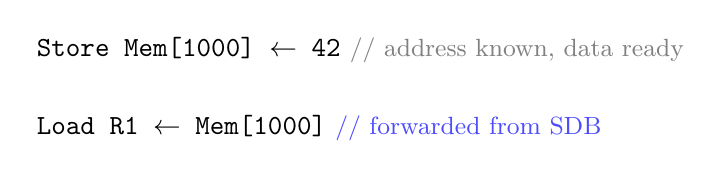
\begin{tikzpicture}[remember picture]
      \node[anchor=west] (store) at (0,0) {\texttt{Store \tikzmark{storemem}Mem[1000] $\leftarrow$ 42} {\small\textcolor{gray}{// address known, data ready}}};
      \node[anchor=west] (load) at (0,-1) {\texttt{Load R1 $\leftarrow$ \tikzmark{loadmem}Mem[1000]} {\small\textcolor{blue!70}{// forwarded from SDB}}};
    \end{tikzpicture}
    \begin{tikzpicture}[remember picture, overlay]
      \draw[->, blue!70, thick] ([xshift=0.5cm, yshift=-2pt]pic cs:storemem) -- node[right, font=\scriptsize] {SDB} ([xshift=0.5cm, yshift=8pt]pic cs:loadmem);
    \end{tikzpicture}
  \end{block}
\end{frame}

\begin{frame}{Data Cache Miss -- Fill Buffers}
\begin{columns}[T]
\begin{column}{0.52\textwidth}
\begin{itemize}
  \item \textbf{Non-blocking D\$:} On miss, continue dispatching subsequent loads
  \begin{itemize}
    \item Blocking cache hurts OOO benefit: hiding miss latency
  \end{itemize}
\end{itemize}
\end{column}
\begin{column}{0.44\textwidth}
\centering
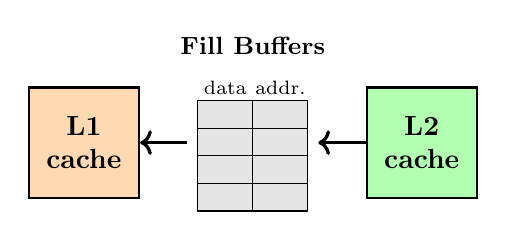
\begin{tikzpicture}[
    cache/.style={draw, thick, minimum width=1.4cm, minimum height=1.4cm, inner sep=2pt, align=center, font=\bfseries},
    fbentry/.style={draw, minimum width=0.7cm, minimum height=0.35cm, fill=gray!20, inner sep=0pt},
    fbheader/.style={minimum width=0.7cm, minimum height=0.35cm, font=\scriptsize, inner sep=0pt},
    ]

    % L1 cache (left)
    \node[cache, fill=orange!30] (l1) at (0, 0) {L1\\cache};

    % Fill Buffers (center) as matrix with header row
    \matrix[right=0.6cm of l1, matrix of nodes,
            row sep=-0.4pt,
            column sep=-0.4pt,
            ampersand replacement=\&,
            label={[font=\small\bfseries]above:Fill Buffers}] (fb) {
        |[fbheader]| data \& |[fbheader]| addr. \\
        |(fb1d)[fbentry]|  \& |(fb1a)[fbentry]|  \\
        |(fb2d)[fbentry]|  \& |(fb2a)[fbentry]|  \\
        |(fb3d)[fbentry]|  \& |(fb3a)[fbentry]|  \\
        |(fb4d)[fbentry]|  \& |(fb4a)[fbentry]|  \\
    };

    % L2 cache (right)
    \node[cache, fill=green!30, right=0.6cm of fb] (l2) {L2\\cache};

    % Arrows: L2 -> FB, FB -> L1
    \draw[->, very thick] (l2.west) -- (l2.west -| fb.east);
    \draw[->, very thick] (fb.west) -- (fb.west -| l1.east);
\end{tikzpicture}
\end{column}
\end{columns}

\begin{itemize}
  \item \textbf{On load miss:}
  \begin{itemize}
    \item Assign a \textbf{Fill Buffer (FB)} entry, issue L2 request
    \item Mark load's result as \textit{invalid}
    \item RS dispatches consumers assuming hit $\rightarrow$ will replay later
  \end{itemize}
  \item More loads can dispatch as long as free FBs exist
  \item Loads to same missed line share the FB entry
\end{itemize}
\end{frame}

\begin{frame}{Data Cache Miss -- Completion}
\begin{itemize}
  \item \textbf{When data returns from L2:}
  \begin{itemize}
    \item Data written to FB; wakeup the load
    \item Load reads directly from FB (no need to wait for D\$ write)
    \item Replay dependent instructions with correct data
  \end{itemize}

  \vspace{0.4cm}

  \item \textbf{Blocked load} (unknown store addr/data):
  \begin{itemize}
    \item Still performs D\$ lookup as \textit{prefetch}
  \end{itemize}
\end{itemize}
\end{frame}

% Updated macro with more flexibility and queue colors
\newcommand{\drawpipelineCustomExt}[9]{%
    % Parameters: 
    % #1: Predict/Fetch color (0=normal, 1=highlight, 2=gray)
    % #2: Decode color
    % #3: Alloc color  
    % #4: Schedule/EX color
    % #5: Retire color
    % #6: IQ queue color (0=green, 1=gray, 2=half gray/half green)
    % #7: uopq queue color (0=green, 1=gray, 2=half gray/half green)
    % #8: RS queue color (0=green, 1=gray, 2=half gray/half green)
    % #9: ROB queue color (0=green, 1=gray, 2=half gray/half green)
    \begin{tikzpicture}[
        remember picture,
        stage/.style={rectangle, draw=black, thick, minimum width=2.2cm, minimum height=0.9cm, font=\footnotesize, fill=orange!40},
        stageHighlight/.style={stage, fill=yellow!60},
        stageGray/.style={stage, fill=gray!30},
        queue/.style={rectangle, draw=black, fill=green!60, minimum width=0.15cm, minimum height=0.7cm},
        queueGray/.style={rectangle, draw=black, fill=gray!30, minimum width=0.15cm, minimum height=0.7cm},
        scale=0.75, transform shape
    ]
        
        % Predict/Fetch
        \ifnum#1=1
            \node[stageHighlight] (fetch) {Predict/Fetch};
        \else
            \ifnum#1=2
                \node[stageGray] (fetch) {Predict/Fetch};
            \else
                \node[stage] (fetch) {Predict/Fetch};
            \fi
        \fi
        
        % IQ queue
        \ifnum#6=1
            \node[queueGray, right=0.1cm of fetch] (iq1) {};
            \node[queueGray, right=0 of iq1] (iq2) {};
            \node[queueGray, right=0 of iq2] (iq3) {};
            \node[queueGray, right=0 of iq3] (iq4) {};
        \else
            \ifnum#6=2
                \node[queueGray, right=0.1cm of fetch] (iq1) {};
                \node[queueGray, right=0 of iq1] (iq2) {};
                \node[queue, right=0 of iq2] (iq3) {};
                \node[queue, right=0 of iq3] (iq4) {};
            \else
                \node[queue, right=0.1cm of fetch] (iq1) {};
                \node[queue, right=0 of iq1] (iq2) {};
                \node[queue, right=0 of iq2] (iq3) {};
                \node[queue, right=0 of iq3] (iq4) {};
            \fi
        \fi
        
        % Decode
        \ifnum#2=1
            \node[stageHighlight, right=0.1cm of iq4] (decode) {Decode};
        \else
            \ifnum#2=2
                \node[stageGray, right=0.1cm of iq4] (decode) {Decode};
            \else
                \node[stage, right=0.1cm of iq4] (decode) {Decode};
            \fi
        \fi
        
        % uopq queue
        \ifnum#7=1
            \node[queueGray, right=0.1cm of decode] (uopq1) {};
            \node[queueGray, right=0 of uopq1] (uopq2) {};
            \node[queueGray, right=0 of uopq2] (uopq3) {};
            \node[queueGray, right=0 of uopq3] (uopq4) {};
        \else
            \ifnum#7=2
                \node[queueGray, right=0.1cm of decode] (uopq1) {};
                \node[queueGray, right=0 of uopq1] (uopq2) {};
                \node[queue, right=0 of uopq2] (uopq3) {};
                \node[queue, right=0 of uopq3] (uopq4) {};
            \else
                \node[queue, right=0.1cm of decode] (uopq1) {};
                \node[queue, right=0 of uopq1] (uopq2) {};
                \node[queue, right=0 of uopq2] (uopq3) {};
                \node[queue, right=0 of uopq3] (uopq4) {};
            \fi
        \fi
        
        % Alloc
        \ifnum#3=1
            \node[stageHighlight, right=0.1cm of uopq4, minimum width=1.5cm] (alloc) {Alloc};
        \else
            \ifnum#3=2
                \node[stageGray, right=0.1cm of uopq4, minimum width=1.5cm] (alloc) {Alloc};
            \else
                \node[stage, right=0.1cm of uopq4, minimum width=1.5cm] (alloc) {Alloc};
            \fi
        \fi
        
        % RS queue
        \ifnum#8=1
            \node[queueGray, right=0.1cm of alloc] (rs1) {};
            \node[queueGray, right=0 of rs1] (rs2) {};
            \node[queueGray, right=0 of rs2] (rs3) {};
            \node[queueGray, right=0 of rs3] (rs4) {};
        \else
            \ifnum#8=2
                \node[queueGray, right=0.1cm of alloc] (rs1) {};
                \node[queueGray, right=0 of rs1] (rs2) {};
                \node[queue, right=0 of rs2] (rs3) {};
                \node[queue, right=0 of rs3] (rs4) {};
            \else
                \node[queue, right=0.1cm of alloc] (rs1) {};
                \node[queue, right=0 of rs1] (rs2) {};
                \node[queue, right=0 of rs2] (rs3) {};
                \node[queue, right=0 of rs3] (rs4) {};
            \fi
        \fi
        
        % Schedule/EX
        \ifnum#4=0
            \node[stage, right=0.1cm of rs4, minimum width=1.8cm] (schedule) {Schedule};
            \node[stage, right=0 of schedule, minimum width=0.8cm] (ex) {EX};
        \fi
         \ifnum#4=1
            \node[stageHighlight, right=0.1cm of rs4, minimum width=1.8cm] (schedule) {Schedule};
            \node[stageHighlight, right=0 of schedule, minimum width=0.8cm] (ex) {EX};
        \fi
        \ifnum#4=2
            \node[stageGray, right=0.1cm of rs4, minimum width=1.8cm] (schedule) {Schedule};
            \node[stageGray, right=0 of schedule, minimum width=0.8cm] (ex) {EX};
        \fi
        \ifnum#4=3
            \node[stage, right=0.1cm of rs4, minimum width=1.8cm] (schedule) {Schedule};
            \node[stageHighlight, right=0 of schedule, minimum width=0.8cm] (ex) {JEU};
        \fi
        
        % ROB queue (shortened to 4 entries)
        \ifnum#9=1
            \node[queueGray, right=0.1cm of ex] (rob1) {};
            \node[queueGray, right=0 of rob1] (rob2) {};
            \node[queueGray, right=0 of rob2] (rob3) {};
            \node[queueGray, right=0 of rob3] (rob4) {};
        \else
            \ifnum#9=2
                \node[queueGray, right=0.1cm of ex] (rob1) {};
                \node[queueGray, right=0 of rob1] (rob2) {};
                \node[queue, right=0 of rob2] (rob3) {};
                \node[queue, right=0 of rob3] (rob4) {};
            \else
                \node[queue, right=0.1cm of ex] (rob1) {};
                \node[queue, right=0 of rob1] (rob2) {};
                \node[queue, right=0 of rob2] (rob3) {};
                \node[queue, right=0 of rob3] (rob4) {};
            \fi
        \fi
        
        % Retire
        \ifnum#5=1
            \node[stageHighlight, right=0.1cm of rob4] (retire) {Retire};
        \else
            \ifnum#5=2
                \node[stageGray, right=0.1cm of rob4] (retire) {Retire};
            \else
                \node[stage, right=0.1cm of rob4] (retire) {Retire};
            \fi
        \fi
        
        % Labels for queues
        \node[font=\scriptsize] at ($(iq1.south)!0.5!(iq4.south)+(0,-0.15)$) {IQ};
        \node[font=\scriptsize] at ($(uopq1.south)!0.5!(uopq4.south)+(0,-0.15)$) {$\mu$opq};
        \node[font=\scriptsize] at ($(rs1.south)!0.5!(rs4.south)+(0,-0.15)$) {RS};
        \node[font=\scriptsize] at ($(rob1.south)!0.5!(rob4.south)+(0,-0.15)$) {ROB};

        % Frontend/Backend backgrounds (on background layer)
        \begin{scope}[on background layer]
            \fill[cyan!10, rounded corners=3pt]
                ($(fetch.north west)+(-0.1,0.1)$) rectangle ($(uopq4.south east)+(0.05,-0.25)$);
            \fill[orange!10, rounded corners=3pt]
                ($(alloc.north west)+(-0.1,0.1)$) rectangle ($(retire.south east)+(0.1,-0.25)$);
        \end{scope}
        \node[font=\footnotesize\sffamily\itshape, text=cyan!60!black]
            at ($(fetch.south west)!0.5!(uopq4.south east)+(0,-0.4)$) {Frontend};
        \node[font=\footnotesize\sffamily\itshape, text=orange!60!black]
            at ($(alloc.south west)!0.5!(retire.south east)+(0,-0.4)$) {Backend};
    \end{tikzpicture}
}

% Original macro for backward compatibility - just calls extended version with all queues green
\newcommand{\drawpipelineCustom}[5]{%
    \drawpipelineCustomExt{#1}{#2}{#3}{#4}{#5}{0}{0}{0}{0}%
}

% Simplified version for basic highlighting
\newcommand{\drawpipeline}[1]{%
    \ifnum#1=0
        \drawpipelineCustom{0}{0}{0}{0}{0}
    \else
        \ifnum#1=1
            \drawpipelineCustom{1}{0}{0}{0}{0}
        \else
            \ifnum#1=2
                \drawpipelineCustom{0}{1}{0}{0}{0}
            \else
                \ifnum#1=3
                    \drawpipelineCustom{0}{0}{1}{0}{0}
                \else
                    \ifnum#1=4
                        \drawpipelineCustom{0}{0}{0}{1}{0}
                    \else
                        \ifnum#1=5
                            \drawpipelineCustom{0}{0}{0}{0}{1}
                        \fi
                    \fi
                \fi
            \fi
        \fi
    \fi
}

\section{OOO Pipeline}

% Slide 1: OOO Machine Pipeline
\begin{frame}{OOO Machine Pipeline}
    \centering
    
    \drawpipeline{0}

    \vspace{0.3cm}
    \begin{itemize}
    \item \textbf{IQ -- Instruction Queue}
    \begin{itemize}
        \item Used mostly in variable length instructions architectures
        \item Smooth the variable number of instruction from a given fetch line
    \end{itemize}
    
    \item \textbf{$\mu$opq}
    \begin{itemize}
        \item Buffer between the fronted and the backend of the machine
        \item Frontend oversupply periods may cover for frontend undersupply periods
    \end{itemize}
    
    \item \textbf{Buffers may be bypassed -- depending on implementation}
    \begin{itemize}
        \item If bypassed, don't cost a cycle when the buffer is empty, e.g., after pipeline flush due to jump misprediction, or following a period of undersupply
    \end{itemize}
  \end{itemize}
\end{frame}

% Slide 2: Pipeline: Predict/Fetch (already provided by user)
\begin{frame}{Pipeline: Predict/Fetch}
    \centering
    \drawpipeline{1}
    
    \vspace{0.5cm}
    \begin{columns}[T]
        \begin{column}{0.9\textwidth}
            \begin{itemize}
                \item Predict the next fetch line
                \item Fetch multiple instruction bytes from the I\$
                \item In case of a variable instruction length architecture (like x86)
                \begin{itemize}
                    \item Length-decode instructions within the fetched instruction bytes
                    \item Write the instructions into an Instruction Queue
                \end{itemize}
            \end{itemize}
        \end{column}
    \end{columns}
\end{frame}

% Slide 3: Pipeline: Decode
\begin{frame}{Pipeline: Decode}
    \centering
    \drawpipeline{2}
    
    \vspace{0.5cm}
    \begin{columns}[T]
        \begin{column}{0.9\textwidth}
            \begin{itemize}
                \item Read multiple instructions from the IQ
                \item Decode the instructions
                \begin{itemize}
                    \item For x86 processors, each instruction is decoded into $\geq$1 $\mu$ops
                    \item $\mu$ops are RISC-like instructions
                \end{itemize}
                \item Write the resulting $\mu$ops into the Instruction Decoder Queue ($\mu$opq)
            \end{itemize}
        \end{column}
    \end{columns}
\end{frame}

% Slide 4: Pipeline: Allocate/Rename
\begin{frame}{Pipeline: Allocate/Rename}
    \centering
    \drawpipeline{3}
    
    \vspace{0.5cm}
    \begin{columns}[T]
        \begin{column}{0.9\textwidth}
            \begin{itemize}
                \item Rename multiple $\mu$ops
                \item Perform port-binding per $\mu$op
                \begin{itemize}
                    \item Select the execution port to which the $\mu$op is dispatched when ready
                \end{itemize}
                \item Allocate ROB/RS entry per $\mu$op
                \begin{itemize}
                    \item If source data is available from ROB or ARF, write data to RS
                    \item Otherwise, mark data not ready in RS
                \end{itemize}
            \end{itemize}
        \end{column}
    \end{columns}
\end{frame}

% Slide 5: Pipeline: EXE
\begin{frame}{Pipeline: EXE}
    \centering
    \drawpipeline{4}
    
    \vspace{0.5cm}
    \begin{columns}[T]
        \begin{column}{0.9\textwidth}
            \textbf{Ready/Schedule}
            \begin{itemize}
                \item Check for data-ready $\mu$ops if the needed port / functional unit are available
                \item Select and dispatch multiple ready $\mu$ops/clock to EXE
            \end{itemize}
            
            \textbf{Write back results into RS/ROB}
            \begin{itemize}
                \item Wake-up $\mu$ops in the RS that are waiting for the results as sources
                \begin{itemize}
                    \item Update data-ready status of these $\mu$ops in the RS
                \end{itemize}
                \item Write back results into the Physical Registers
                \item Reclaim RS entries
            \end{itemize}
        \end{column}
    \end{columns}
\end{frame}

% Slide 6: Pipeline: Retire
\begin{frame}{Pipeline: Retire}
    \centering
    \drawpipeline{5}

    \vspace{0.2cm}
    \begin{columns}[T]
        \begin{column}{0.9\textwidth}
            \textbf{Retire oldest $\mu$ops in the ROB}
            \begin{itemize}
                \item A $\mu$op may retire if
                \begin{itemize}
                    \item Its ``executed'' bit is set
                    \item It is not marked with an exception / fault
                    \item All preceding $\mu$ops are eligible for retirement
                \end{itemize}
                \item Commit results from the Physical Register to the Arch Register
                \item Reclaim the ROB entry
            \end{itemize}
            
            \textbf{In case of exception / fault}
            \begin{itemize}
                \item Flush the pipeline and handle the exception / fault
                \item Restart the program
            \end{itemize}
        \end{column}
    \end{columns}
\end{frame}

\section{Misprediction Recovery}

% Slide: Misprediction Recovery Overview
\begin{frame}[label=misprediction-recovery]{Misprediction Recovery -- Two Approaches}
    \centering
    \vspace{0.5cm}

    \small
    \begin{tabularx}{\textwidth}{@{} l X X @{}}
        \toprule
        & \textbf{Flush at Retire} & \textbf{Flush at Execute} \\
        \midrule
        \textbf{When recover} & \textcolor{red!70!black}{When mispredicted jump retires} & \textcolor{green!50!black}{When misprediction detected} \\[0.2cm]
        \textbf{What's flushed} & \textcolor{red!70!black}{Entire pipeline} & \textcolor{green!50!black}{Frontend only (initially)} \\[0.2cm]
        \textbf{Penalty} & \textcolor{red!70!black}{High (wait for retire)} & \textcolor{green!50!black}{Lower (act immediately)} \\[0.2cm]
        \textbf{Complexity} & \textcolor{green!50!black}{Simple} & \textcolor{red!70!black}{Higher (needs checkpointing)} \\[0.2cm]
        \textbf{Wrong-path work} & Executes until retire & Executes until retire \\
        \bottomrule
    \end{tabularx}

    \vspace{0.5cm}
    \begin{itemize}
        \item Both approaches detect misprediction at execute
        \item Difference: when to start fetching from correct path
    \end{itemize}
\end{frame}

% Slide: Flush at Retire: Jump Executed
\begin{frame}{Flush at Retire: Jump Executed}
    \centering
    \drawpipelineCustom{0}{0}{0}{3}{0}

    \vspace{0.5cm}
    \begin{itemize}
        \item Misprediction detected --- mark jump as mispredicted in ROB
        \item Pipeline continues filling with wrong-path instructions
        \item No recovery action yet --- wait for jump to retire
    \end{itemize}
\end{frame}

% Slide 9: Flush at Retire: Jump Retires
\begin{frame}{Flush at Retire: Jump Retires}
    \vspace{0.5cm}
    \centering
    \drawpipelineCustomExt{2}{2}{2}{2}{2}{1}{1}{1}{1}

    % Add flush arrow and text using node positions from the macro
    \begin{tikzpicture}[overlay, remember picture]
        \draw[->, red, ultra thick] (retire.north) -- ++(0,0.8) -|
          node[red, font=\bfseries\small, below, near start] {Flush} (fetch.north)
          node[black, font=\scriptsize, near end, left, align=right] {Redirect Fetch\\+ update BPU};
    \end{tikzpicture}

    \vspace{0.3cm}
    \begin{itemize}
        \item Flush entire pipeline (all instructions are wrong-path)
        \item Reset rename map to architectural registers
        \item Redirect fetch to correct path
    \end{itemize}
\end{frame}

% Slide: Flush at Execute: Jump Executed
\begin{frame}{Flush at Execute: Jump Executed}
    \vspace{0.5cm}
    \centering
    \drawpipelineCustomExt{2}{2}{0}{3}{0}{1}{1}{0}{0}

    % Add Flush arrow and labels
    \begin{tikzpicture}[overlay, remember picture]
        \draw[->, red, ultra thick] (ex.north) -- ++(0,0.8) -|
          node[red, font=\bfseries\small, below, near start] {Flush} (fetch.north)
          node[black, font=\scriptsize, near end, left, align=right] {Redirect Fetch\\+ update BPU};
        % draw red line left of alloc
        \draw[red, ultra thick] ([yshift=-1mm]alloc.south west) -- ([yshift=1mm]alloc.north west);
    \end{tikzpicture}

    \vspace{0.3cm}
    \begin{itemize}
        \item Flush frontend and redirect to correct path
        \item Block allocation (rename map corrupted)
        \item OOO continues --- wrong-path instructions still execute
        \item Block younger jumps (executed OOO) from triggering flushes
        \item Caveat: ``correct'' path may still be wrong (older jump/exception)
    \end{itemize}
\end{frame}

% Slide: Flush at Execute: Jump Retires
\begin{frame}{Flush at Execute: Jump Retires}
    \vspace{0.5cm}
    \centering
    \drawpipelineCustomExt{0}{0}{2}{2}{2}{0}{0}{1}{1}

    % Clear arrow
    \begin{tikzpicture}[overlay, remember picture]
        \draw[->, red, ultra thick]
          (retire.north) -- ++(0,0.8) -| node[red, font=\bfseries\small, below, near start] {Flush} (alloc.north);
    \end{tikzpicture}

    \vspace{0.3cm}
    \begin{itemize}
        \item Flush OOO backend (only wrong-path instructions remain)
        \item Reset rename map to architectural registers
        \item Unblock allocation for correct-path instructions
    \end{itemize}
\end{frame}

% Slide 14: Periodic Checkpoints
\begin{frame}{Periodic Checkpoints}
  \begin{columns}[T]
    \begin{column}{0.67\textwidth}
      \begin{itemize}\setlength{\itemsep}{0.15cm}
        \item \textbf{Allow allocation from correct path before mispredicted jump retires}

        \item \textbf{Periodically checkpoint the Renamer}
        \begin{itemize}\setlength{\itemsep}{0pt}
          \item Snapshot of renaming map every N instructions
          \item Per-jump snapshots too expensive
        \end{itemize}

        \item \textbf{On misprediction:}
        \begin{itemize}\setlength{\itemsep}{0pt}
          \item Flush frontend, fetch from correct path
          \item Selectively flush younger instructions from ROB/RS
          \item Recover Renamer to latest checkpoint before the jump
          \item Re-rename: replay instructions from checkpoint to jump
          \item Resume allocation from correct path
        \end{itemize}
      \end{itemize}
    \end{column}

    \begin{column}{0.33\textwidth}
      \centering
      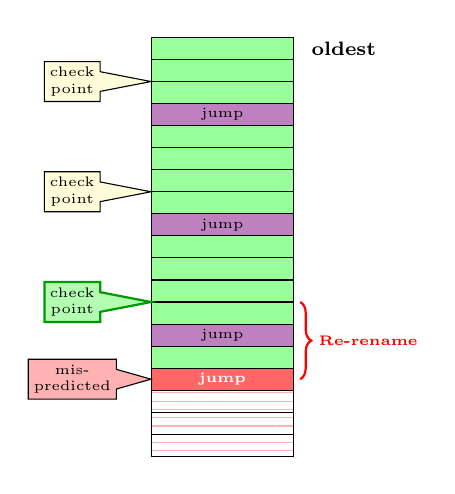
\begin{tikzpicture}[font=\tiny,
        N/.style={draw, fill=green!40, minimum width=1.8cm, minimum height=0.28cm, inner sep=1pt},
        J/.style={N, fill=violet!50},
        M/.style={N, fill=red!60},
        S/.style={N, fill=red!20, pattern=horizontal lines, pattern color=red!30},
        chk/.style={draw, fill=yellow!15, align=center, inner sep=2pt, rectangle callout},
        chkA/.style={chk, fill=green!30, draw=green!60!black, thick}
      ]
        \matrix[matrix of nodes, ampersand replacement=\&, row sep=-\pgflinewidth,
          nodes={minimum width=1.8cm, minimum height=0.28cm, inner sep=1pt}
        ] (m) {
          |[N]| \\
          |[N]| \\
          |[N]| \\
          |[J]| jump \\
          |[N]| \\
          |[N]| \\
          |[N]| \\
          |[N]| \\
          |[J]| jump \\
          |[N]| \\
          |[N]| \\
          |[N]| \\
          |[N]| \\
          |[J]| jump \\
          |[N]| \\
          |[M, text=white, font=\tiny\bfseries]| jump \\
          |[S]| \\
          |[S]| \\
          |[S]| \\
        };
        % "oldest" label (to the right)
        \node[right=0.1cm of m-1-1.east, font=\scriptsize\bfseries] {oldest};
        % Periodic checkpoints between entries (every 5 rows starting after row 2)
        \node[chk, callout absolute pointer={($(m-2-1.south west)!0.5!(m-3-1.north west)$)}] at ($(m-2-1.south west)!0.5!(m-3-1.north west)+(-1.0,0)$) {check\\point};
        \node[chk, callout absolute pointer={($(m-7-1.south west)!0.5!(m-8-1.north west)$)}] at ($(m-7-1.south west)!0.5!(m-8-1.north west)+(-1.0,0)$) {check\\point};
        \node[chkA, callout absolute pointer={($(m-12-1.south west)!0.5!(m-13-1.north west)$)}] at ($(m-12-1.south west)!0.5!(m-13-1.north west)+(-1.0,0)$) {check\\point};
        % Misprediction callout (on the left like checkpoints)
        \node[draw, fill=red!30, rectangle callout, callout absolute pointer={(m-16-1.west)}, font=\tiny, align=center, inner sep=2pt]
          at ($(m-16-1.west)+(-1.0,0)$) {mis-\\predicted};
        % Re-rename brace on the right (from checkpoint between 12-13 to mispredicted jump at row 16)
        \draw[decorate, decoration={brace, amplitude=4pt}, thick, red]
          ($(m-12-1.south east)!0.5!(m-13-1.north east)+(0.08,0)$) -- ($(m-16-1.east)+(0.08,0)$)
          node[midway, right=3pt, font=\tiny\bfseries, text=red] {Re-rename};
      \end{tikzpicture}
    \end{column}
  \end{columns}
\end{frame}

\begin{frame}{Checkpoints: Jump Executed}
    \centering
    \drawpipelineCustomExt{0}{0}{0}{3}{0}{1}{1}{2}{2}

    % Add BPU Update and Clear labels
    \begin{tikzpicture}[overlay, remember picture]
        \draw[->, red, ultra thick] (ex.north) -- ++(0,0.8) -|
          node[red, font=\bfseries\small, below, near start] {Flush} (fetch.north)
          node[black, font=\scriptsize, near end, left, align=right] {update BPU};
    \end{tikzpicture}

    \vspace{0.5cm}
    \begin{itemize}
        \item Flush frontend and redirect to correct path
        \item \textcolor{orange}{Flush younger instructions in OOO} (by ROB age comparison)
        \item Block allocation until Renamer recovered
    \end{itemize}
\end{frame}

% Slide: Checkpoints: Recovering Renamer
\begin{frame}{Checkpoints: Recovering Renamer}
    \vspace{0.5cm}
    \centering
    \drawpipelineCustomExt{2}{2}{2}{0}{0}{1}{1}{2}{2}

    \begin{tikzpicture}[overlay, remember picture]
        \draw[red, ultra thick] ([yshift=-1mm]alloc.south west) -- ([yshift=1mm]alloc.north west);
    \end{tikzpicture}

    \vspace{0.3cm}
    \begin{itemize}
        \item Restore Renamer from latest checkpoint before the jump
        \item Re-rename instructions from checkpoint to jump
        \item Frontend fetches correct path (blocked at allocation)
    \end{itemize}
\end{frame}

% Slide: Checkpoints: Recovery Complete
\begin{frame}{Checkpoints: Recovery Complete}
    \vspace{0.5cm}
    \centering
    \drawpipelineCustomExt{0}{0}{1}{0}{0}{0}{0}{2}{2}

    \vspace{0.5cm}
    \begin{itemize}
        \item Renamer restored --- unblock allocation
        \item Correct-path instructions now flow through
    \end{itemize}
\end{frame}

% Backup
\begin{frame}{Backup}
\end{frame}

\begin{frame}{ROB Designs: Merged vs Separate Register File}
  \begin{columns}[T]
    \begin{column}{0.48\textwidth}
      \centering
      \textbf{Merged RF + ROB Status}\\
      {\small\textit{P6 / Pentium III}}
      \vspace{0.15cm}

      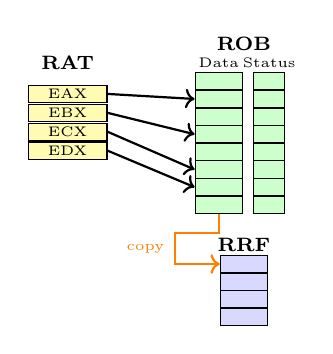
\begin{tikzpicture}[font=\tiny, scale=0.8,
        rat/.style={draw, fill=yellow!30, minimum width=1.0cm, minimum height=0.22cm, inner sep=1pt},
        robcell/.style={draw, fill=green!20, minimum width=0.6cm, minimum height=0.22cm, inner sep=1pt},
        rrfcell/.style={draw, fill=blue!15, minimum width=0.6cm, minimum height=0.22cm, inner sep=1pt},
      ]
        % RAT
        \node[font=\scriptsize\bfseries] at (-1.5, 2.2) {RAT};
        \foreach \i/\reg in {0/EAX, 1/EBX, 2/ECX, 3/EDX} {
          \node[rat] (rat\i) at (-1.5, 1.7-\i*0.3) {\reg};
        }

        % ROB with Data and Status
        \node[font=\scriptsize\bfseries] at (1.3, 2.5) {ROB};
        \node[font=\tiny] at (0.9, 2.2) {Data};
        \node[font=\tiny] at (1.7, 2.2) {Status};
        \foreach \i in {0,...,7} {
          \node[robcell] (robd\i) at (0.9, 1.9-\i*0.28) {};
          \node[robcell, minimum width=0.4cm] (robs\i) at (1.7, 1.9-\i*0.28) {};
        }

        % RRF
        \node[font=\scriptsize\bfseries] (rrfLabel) at (1.3, -0.7) {RRF};
        \foreach \i in {0,...,3} {
          \node[rrfcell] (rrf\i) at (1.3, -1.0-\i*0.28) {};
        }

        % Arrows from RAT to ROB
        \draw[->, thick] (rat0.east) -- (robd1.west);
        \draw[->, thick] (rat1.east) -- (robd3.west);
        \draw[->, thick] (rat2.east) -- (robd5.west);
        \draw[->, thick] (rat3.east) -- (robd6.west);

        % Arrow from ROB to RRF (copy on retire) - routed left of RRF
        \draw[->, orange, thick] (robd7.south) |- ++(-0.7,-0.3) |- (rrf0.west)
          node[pos=0.25, left, font=\tiny, text=orange] {copy};
      \end{tikzpicture}

      \vspace{0.2cm}
      \begin{itemize}\setlength{\itemsep}{0pt}\footnotesize
        \item ROB holds speculative values
        \item RRF holds committed values
        \item \textcolor{orange}{Copy data on retirement}
      \end{itemize}
    \end{column}

    \begin{column}{0.48\textwidth}
      \centering
      \textbf{Separate RF + Retirement RAT}\\
      {\small\textit{NetBurst / Pentium 4}}
      \vspace{0.15cm}

      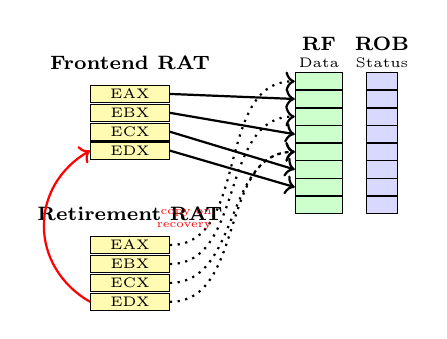
\begin{tikzpicture}[font=\tiny, scale=0.8,
        rat/.style={draw, fill=yellow!30, minimum width=1.0cm, minimum height=0.22cm, inner sep=1pt},
        rfcell/.style={draw, fill=green!20, minimum width=0.6cm, minimum height=0.22cm, inner sep=1pt},
        robcell/.style={draw, fill=blue!15, minimum width=0.4cm, minimum height=0.22cm, inner sep=1pt},
      ]
        % Frontend RAT
        \node[font=\scriptsize\bfseries] at (-1.5, 2.5) {Frontend RAT};
        \foreach \i/\reg in {0/EAX, 1/EBX, 2/ECX, 3/EDX} {
          \node[rat] (frat\i) at (-1.5, 2.0-\i*0.3) {\reg};
        }

        % Retirement RAT (moved up slightly)
        \node[font=\scriptsize\bfseries] at (-1.5, 0.1) {Retirement RAT};
        \foreach \i/\reg in {0/EAX, 1/EBX, 2/ECX, 3/EDX} {
          \node[rat] (rrat\i) at (-1.5, -0.4-\i*0.3) {\reg};
        }

        % RF (Data) and ROB (Status)
        \node[font=\scriptsize\bfseries] at (1.5, 2.8) {RF};
        \node[font=\scriptsize\bfseries] at (2.5, 2.8) {ROB};
        \node[font=\tiny] at (1.5, 2.5) {Data};
        \node[font=\tiny] at (2.5, 2.5) {Status};
        \foreach \i in {0,...,7} {
          \node[rfcell] (rf\i) at (1.5, 2.2-\i*0.28) {};
          \node[robcell] (rob\i) at (2.5, 2.2-\i*0.28) {};
        }

        % Arrows from Frontend RAT to RF (solid)
        \draw[->, thick] (frat0.east) -- (rf1.west);
        \draw[->, thick] (frat1.east) -- (rf3.west);
        \draw[->, thick] (frat2.east) -- (rf5.west);
        \draw[->, thick] (frat3.east) -- (rf6.west);

        % Arrows from Retirement RAT to RF (dotted)
        \draw[->, dotted, thick] (rrat0.east) to[out=0,in=180] (rf0.west);
        \draw[->, dotted, thick] (rrat1.east) to[out=0,in=180] (rf2.west);
        \draw[->, dotted, thick] (rrat2.east) to[out=0,in=180] (rf4.west);
        \draw[->, dotted, thick] (rrat3.east) to[out=0,in=180] (rf4.west);

        % Recovery arrow from Retirement RAT to Frontend RAT (west to west, curved left)
        \draw[->, red, thick] (rrat3.west) to[out=150,in=-150, looseness=1.2] (frat3.west)
          node[pos=0.5, left=2pt, font=\tiny, text=red, align=right] {copy on\\recovery};
      \end{tikzpicture}

      \vspace{0.2cm}
      \begin{itemize}\setlength{\itemsep}{0pt}\footnotesize
        \item RF holds \textbf{all} values (speculative + committed)
        \item ROB only tracks status (no data)
        \item \textcolor{green!50!black}{No copy on retirement!}
        \item \textcolor{red}{Copy RRAT$\to$RAT on recovery}
      \end{itemize}
    \end{column}
  \end{columns}
\end{frame}

\begin{frame}{The Pentium® Processor (1993)}
  \begin{itemize}
    \item \textbf{Fetch and decode 2 instructions per cycle}
    
    \item \textbf{At decode stage decide on \emph{pairing}:} can the two instructions be executed in parallel
    
    \item \textbf{Pairing decision is based on:}
    \begin{itemize}
      \item \textcolor{blue}{Data dependencies}: 2nd instruction must be independent of 1st
      \begin{itemize}
        \item If the 1st instruction produces data needed by the 2nd instruction, the 2nd instruction cannot be executed in parallel to the 1st instruction
      \end{itemize}
      
      \item \textcolor{blue}{Resources}: U-pipe and V-pipe are not symmetric (save HW)
      \begin{itemize}
        \item Common instructions can execute on either pipe
        \item Some instructions can execute only on the U-pipe
        \item V-pipe can run a subset of the instructions that can run on U-pipe
        \item If the 2nd instruction requires the U-pipe, it cannot pair
        \item Some instructions use resources of both pipes (and therefore cannot pair)
      \end{itemize}
    \end{itemize}
  \end{itemize}
  
  \begin{center}
    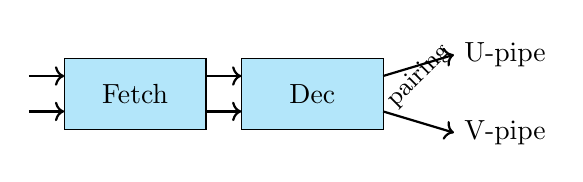
\begin{tikzpicture}[scale=0.9]
      \draw[->, thick] (-0.5,0) -- (0,0);
      \draw[->, thick] (-0.5,-0.5) -- (0,-0.5);
      \draw[fill=cyan!30] (0,-0.75) rectangle (2,0.25) node[midway] {Fetch};
      \draw[->, thick] (2,0) -- (2.5,0);
      \draw[->, thick] (2,-0.5) -- (2.5,-0.5);
      \draw[fill=cyan!30] (2.5,-0.75) rectangle (4.5,0.25) node[midway] {Dec};
      \node[rotate=45] at (5,0) {\small pairing};
      \draw[->, thick] (4.5,0) -- (5.5,0.3) node[right] {U-pipe};
      \draw[->, thick] (4.5,-0.5) -- (5.5,-0.8) node[right] {V-pipe};
    \end{tikzpicture}
  \end{center}
\end{frame}


\end{document}
